\documentclass[11pt]{article}
\usepackage[utf8]{inputenc}
\usepackage[french]{babel}
\usepackage{graphicx}
\usepackage{caption}
\usepackage{fancyhdr} 
\usepackage{float}
\usepackage{lastpage}
\usepackage{amsmath}
%\usepackage{todonotes}
\usepackage{dirtree}
\usepackage{caption}
\usepackage{subcaption}

\graphicspath{{./Images/}}

\renewcommand{\thesection}{\Roman{section}. }
\renewcommand{\thesubsection}{\Roman{section}.\arabic{subsection}}
\renewcommand{\thesubsubsection}{\Roman{section}.\arabic{subsection}.\alph{subsubsection} }

\setlength{\hoffset}{-18pt}
\setlength{\oddsidemargin}{0pt}
\setlength{\evensidemargin}{0pt}
\setlength{\marginparwidth}{54pt}
\setlength{\textwidth}{494pt}
\setlength{\voffset}{-45pt}
\setlength{\marginparsep}{7pt}
\setlength{\topmargin}{0pt}
\setlength{\headheight}{13pt}
\setlength{\headsep}{15pt}
\setlength{\textheight}{680pt}

\pagestyle{fancy}

\renewcommand{\headrulewidth}{1pt}
\fancyhead[L]{\textsc{Quoridor}}
\fancyhead[C]{}
\fancyhead[R]{\leftmark}

\renewcommand{\footrulewidth}{1pt}
\fancyfoot[L]{Rapport de projet}
\fancyfoot[C]{\textbf{\thepage/\pageref{LastPage}}}
\fancyfoot[R]{Equipe 12818}


\title{Rapport Projet}
\date{2020-2021}


\begin{document}





\begin{titlepage}
\centering

\includegraphics[scale=0.4]{enseirb.png}
\\
\vspace*{1\baselineskip}
\LARGE{\textsc{Rapport de projet}}
\vspace*{0.8\baselineskip}
\rule{1\linewidth}{1pt}

\huge{\textbf{QUORIDOR}}
\vspace*{1\baselineskip}
\rule{1\linewidth}{1pt}
\vspace*{1\baselineskip}
\LARGE{\textsc{Filière Informatique - Semestre 6}}
\\

\large{\today}
\vspace*{3\baselineskip}
\\
\centering
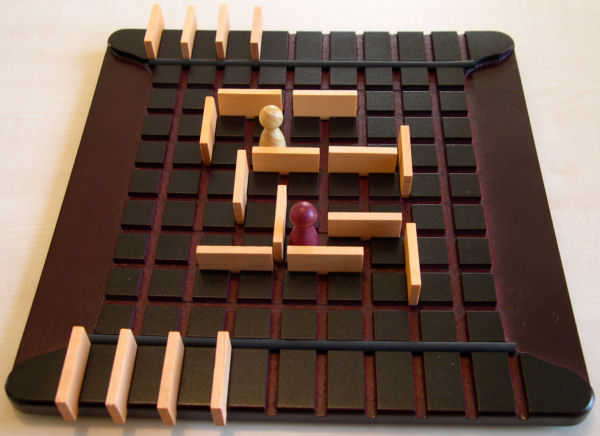
\includegraphics[scale=1.4]{quoridor.png}
\\
\vspace*{4\baselineskip}

\begin{minipage}[b]{0.40\linewidth}
        \flushleft 
        \large
        Auteurs : 
        \\
        \textsc{Choura} Alexandre
        \\
        \textsc{Guerin} Léo
        \\
        \textsc{Marais} Lucas
        \\
        \textsc{Sornay} Jean-François
    \end{minipage} \hfill
    \begin{minipage}[b]{0.40\linewidth}
        \flushright 
        \large 
        Encadrants : 
        \\
        \textsc{Renault} David
        \\
        \textsc{Eyrolles} Georges
    \end{minipage} \hfill

\end{titlepage}

\newpage

\tableofcontents

\newpage

\section{Introduction}
Le but de ce projet est d'avoir une première approche des enjeux, des difficultés et des solutions liées à la mise en oeuvre d'une architecture clients-serveur.
Pour ce projet, cette thématique est abordée par le développement du jeu de stratégie combinatoire Quoridor à travers une telle architecture dans le langage C.
Le serveur faisant ici office d'arbitre ainsi que d'interprète entre les clients qui, eux, sont appelés des "joueurs" et sont en réalité différentes implémentations de stratégie.

\subsection{Brève introduction au jeu Quoridor}
Quoridor est un jeu se jouant sur un plateau composé de tuiles carrées. Chaque joueur est représenté par un pion et peut commencer sur des positions prédéfinies. L'objectif est d'être le premier joueur à atteindre n'importe laquelle des positions prédéfinies adverses.

\vspace{4mm}

Pour cela, chaque tour, les joueurs peuvent, les uns après les autres, effectuer une des deux actions possibles : "se déplacer" ou "poser un mur".

\vspace{4mm}

Comme son nom l'indique, l'action "se déplacer" revient à déplacer son pion sur les cases adjacentes par rapport à sa position actuelle. Dans certaines configurations de jeu, le joueur peut passer outre cette condition d'adjacence afin de se déplacer sur une case en diagonale ou par-dessus celle du joueur adverse. Ces différents déplacements possibles sont visibles en figure \ref{fig:correct_move}.

\begin{figure}[H]
    \centering
    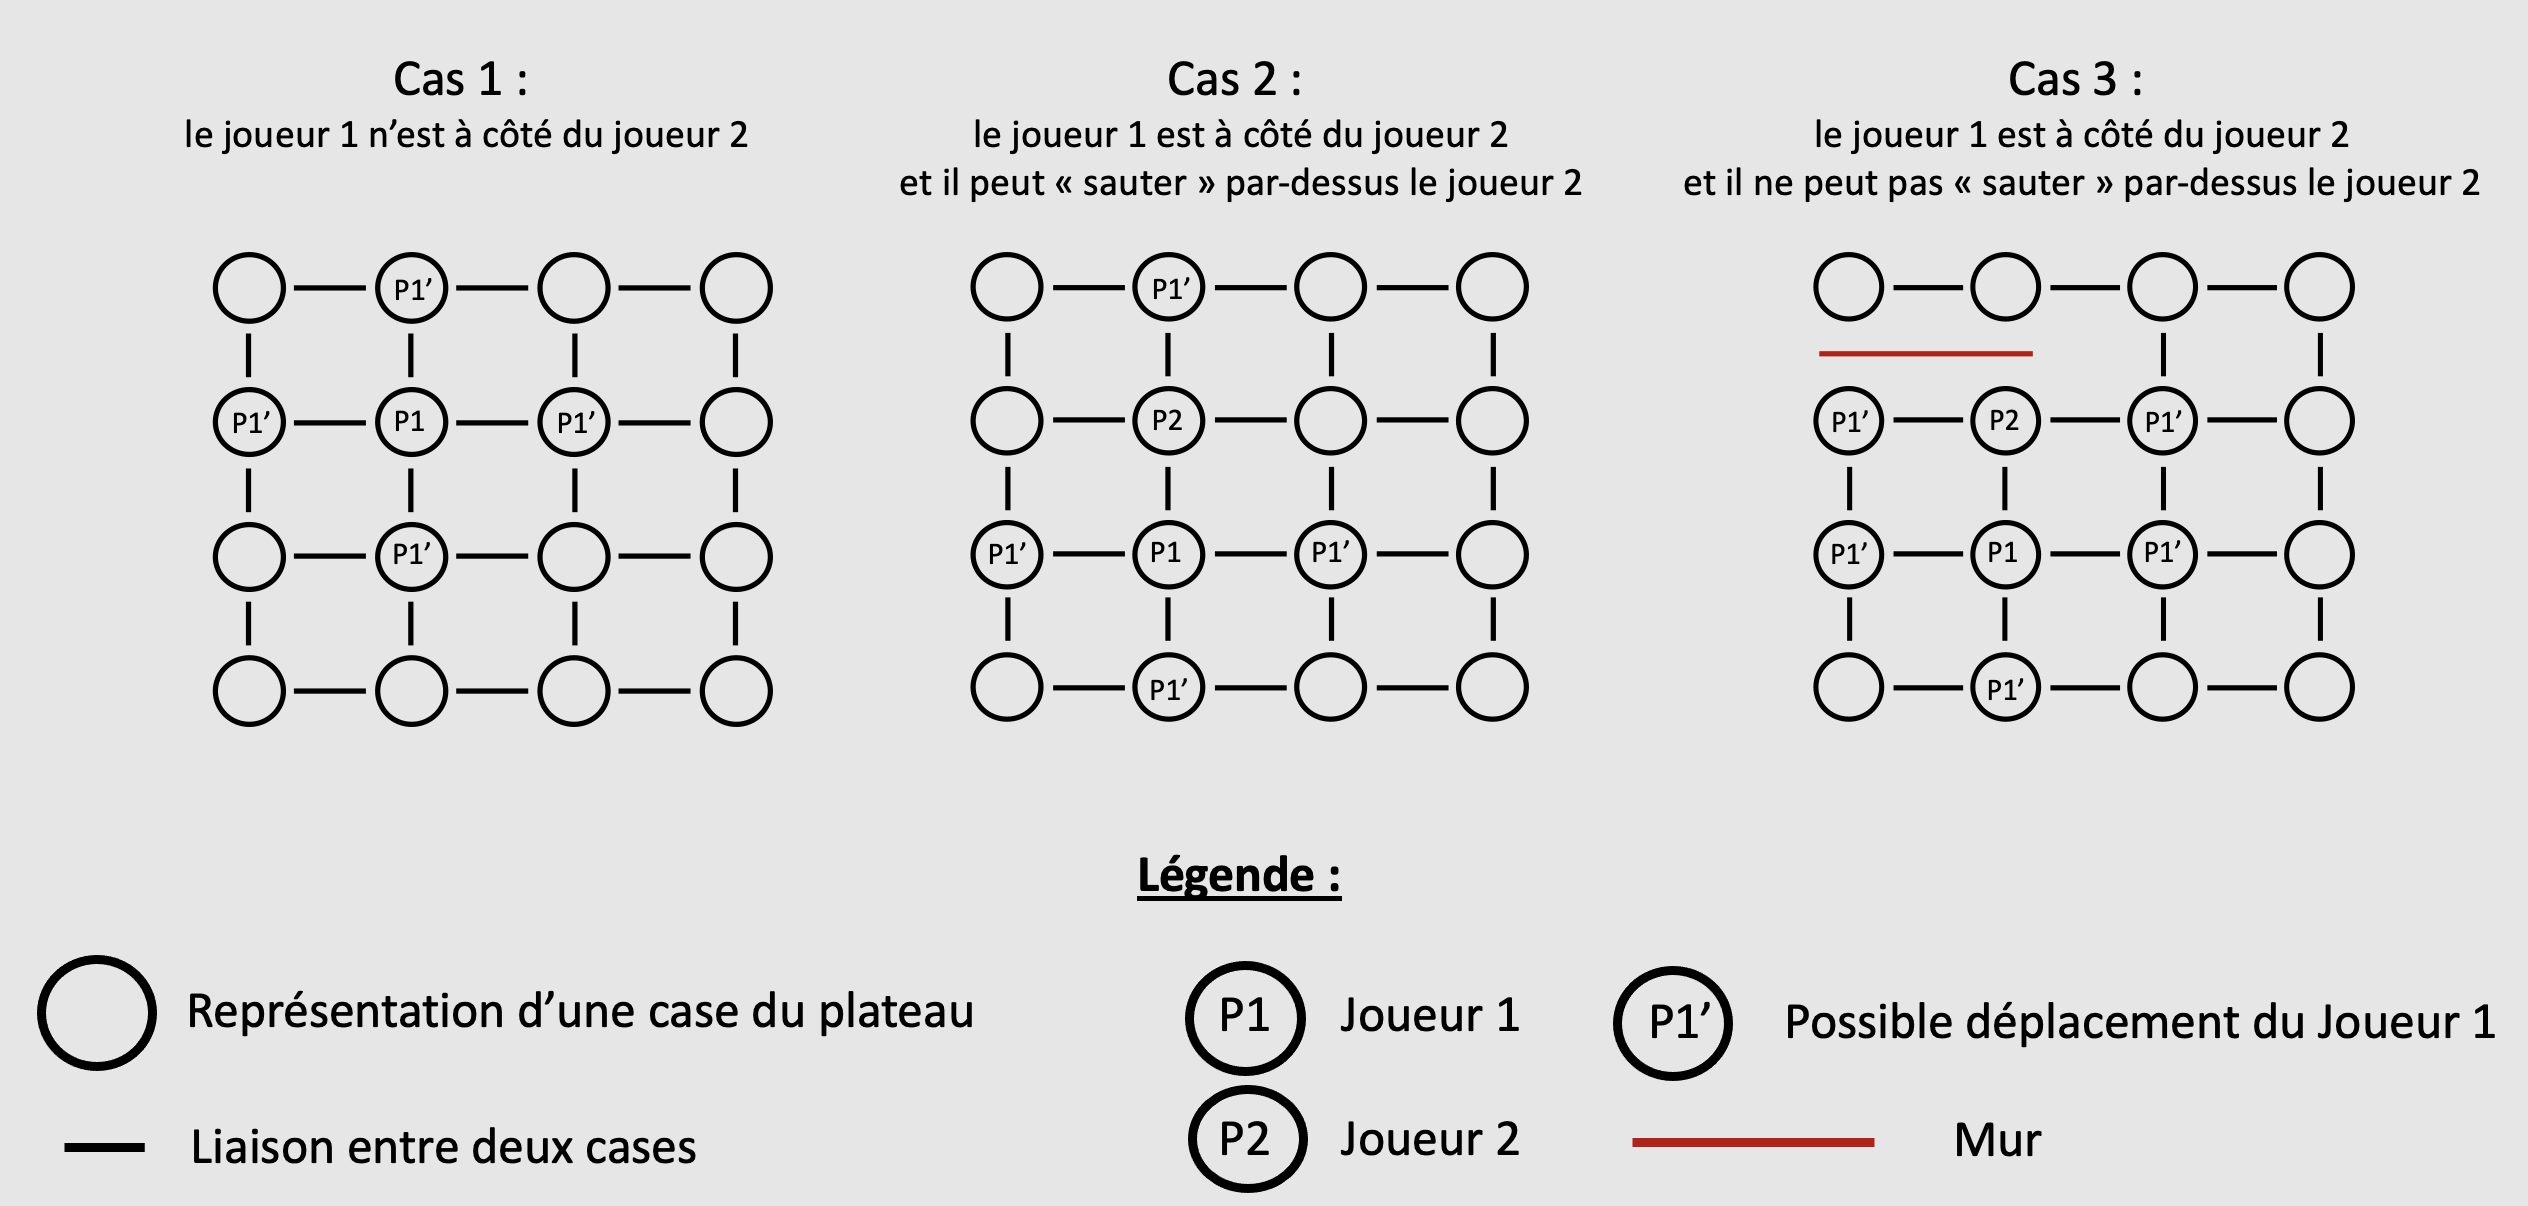
\includegraphics[width=\linewidth]{correct_move.png}
    \caption{Schéma des déplacements possibles d'un joueur}
    \label{fig:correct_move}
\end{figure}

L'action de "poser un mur", équivaut à retirer la relation d'adjacence entre plusieurs cases du plateau de jeu afin de restreindre les déplacements des joueurs. Toutefois, cette action possède quelques restrictions. En effet, les murs peuvent être représentés par une ligne droite de longueur fixe équivalente à deux case. Un mur ne peut donc ni sortir du plateau ni former d'angle droit à partir de lui-même. De plus, la pose d'un mur ne peut empêcher définitivement un joueur d'atteindre au moins une des positions gagnantes. Plusieurs exemples de placements autorisés de murs ainsi que des placements de murs interdits sont représentés par les figures \ref{fig:correct_wall} et \ref{fig:incorrect_wall}.

\begin{figure}[H]
    \centering
    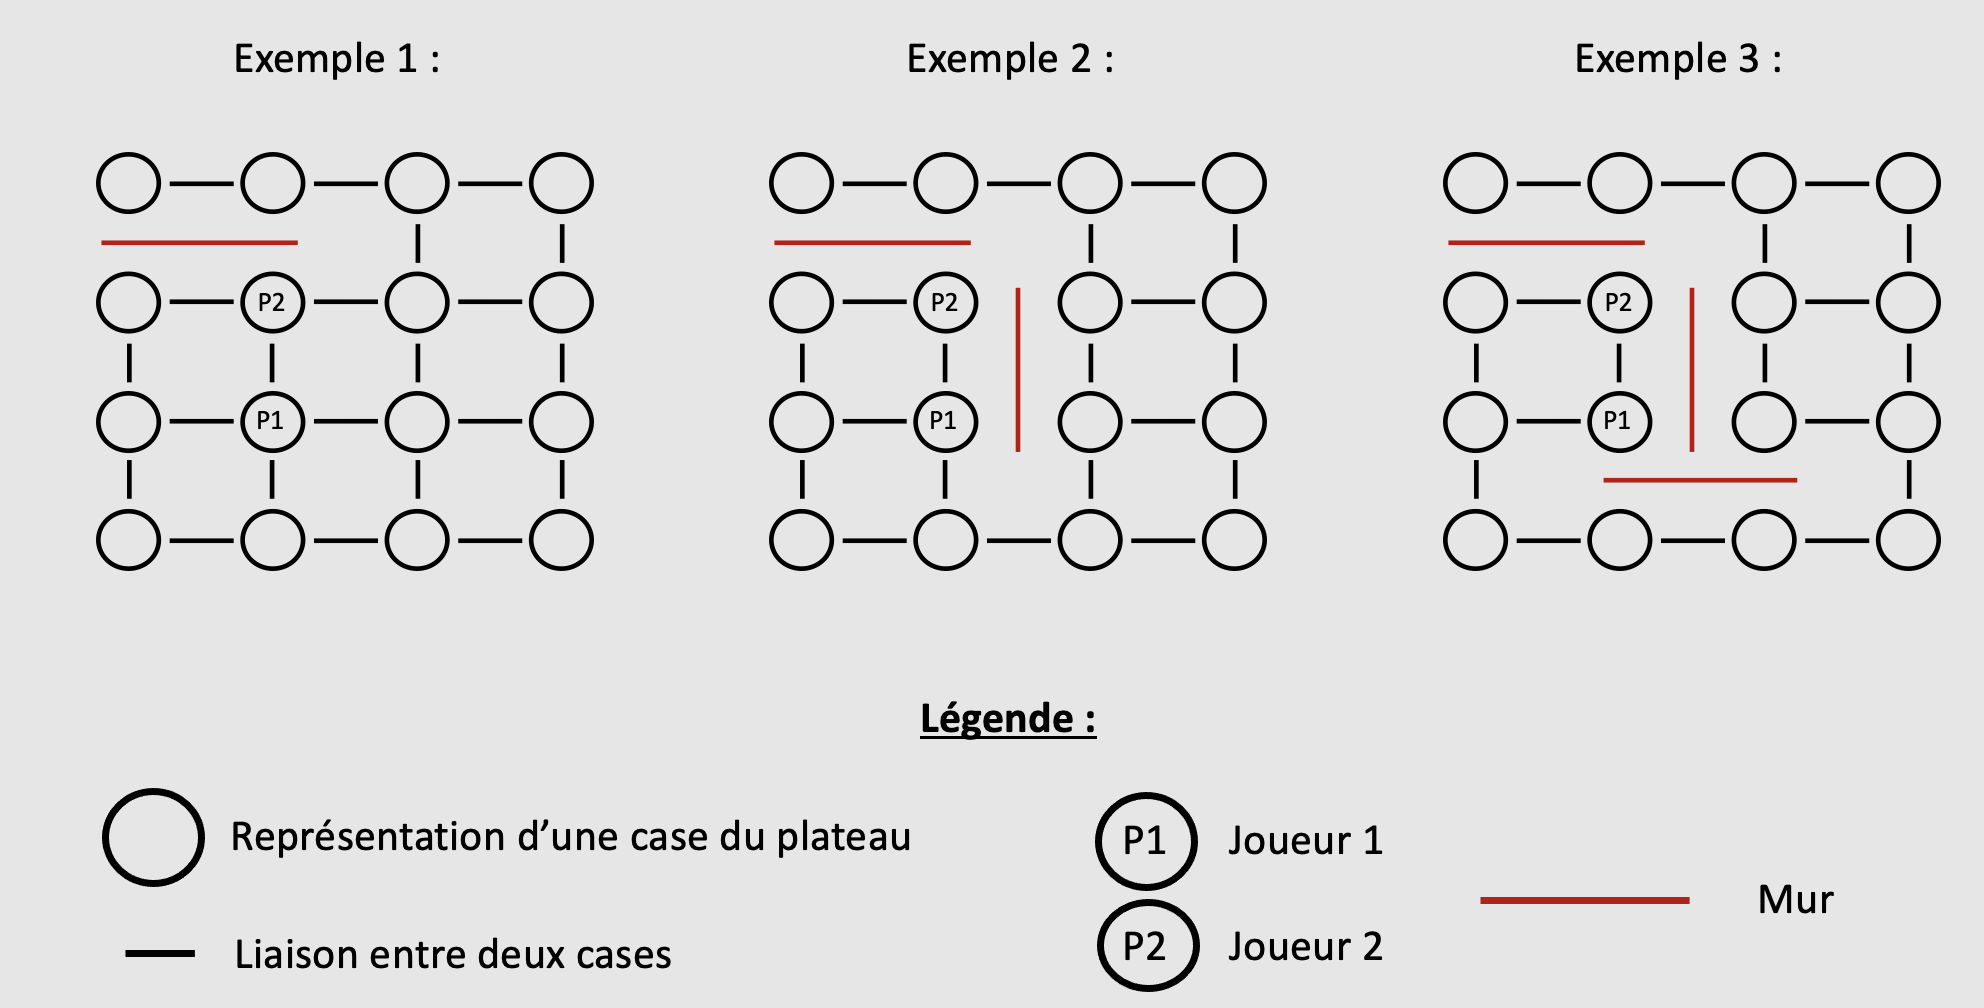
\includegraphics[width=\linewidth]{correct_wall.png}
    \caption{Exemples de placements autorisés de murs}
    \label{fig:correct_wall}
\end{figure}


\begin{figure}[H]
    \centering
    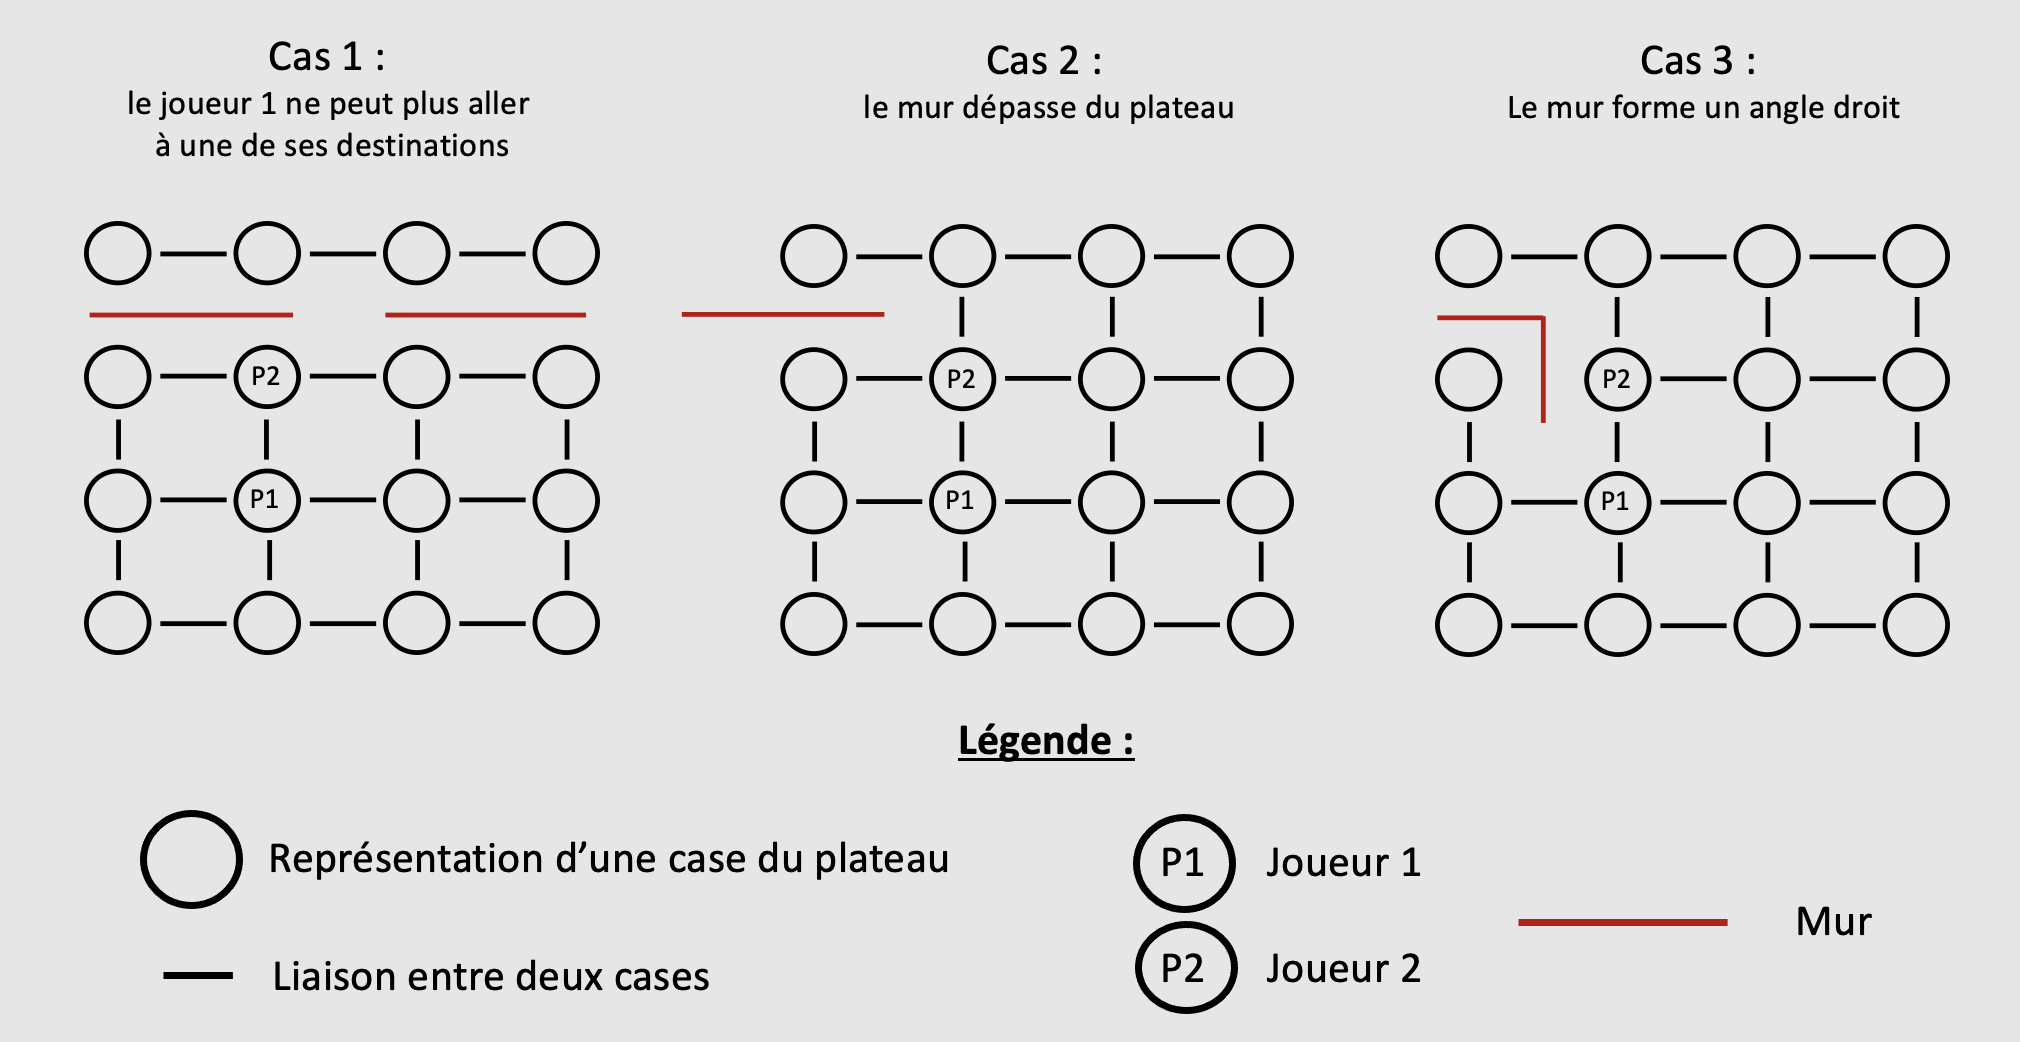
\includegraphics[width=\linewidth]{incorrect_wall.png}
    \caption{Exemples de placements interdits de murs}
    \label{fig:incorrect_wall}
\end{figure}

\subsection{Problématiques et contraintes du projet}

Tel qu'évoqué précédemment, la problématique principale est de mettre en place un protocole de communication entre deux types d'entités, ici nommés serveur et joueurs. Pour être plus précis, il s'agit de développer et d'implanter une interface de communication entre un joueur et le serveur, et vice-versa. Cette interface nous a été imposée et correspond à l'obligation de réaliser quatre fonctions pour chaque joueur afin de communiquer avec le serveur : une fonction afin d'obtenir le nom du joueur, une fonction d'initialisation, une fonction permettant à celui-ci de réaliser une action et une fonction marquant la fin du jeu. Cette interface contraint également le type de données transmises entre un serveur et les différents clients.

La problématique secondaire de ce projet est celle du développement de stratégies rapides en temps et efficaces, c'est-à-dire ayant une forte probabilité d'être gagnante. Les contraintes de cette problématique sont donc le type de stratégie mise en place et le temps de calcul lors du choix d'action à effectuer par un joueur.

\vspace{4mm}

Dans ce rapport, nous présentons dans un premier temps, notre vision d'un serveur et la manière dont nous l'avons pensé. Dans un second temps, nous présentons de la même manière les différents joueurs.
Nous évoquons ensuite l'architecture que nous avons mise en place pour le projet. Nous enchaînons avec l'explication de notre méthodologie de test et leurs mises en place. Enfin, nous énoncerons notre gestion de projet avant de conclure en revenant brièvement sur la résolution des différentes problématiques.

\newpage
\section{Serveur}

Nous présentons dans cette section, les différentes thématiques que nous avons abordées et auxquelles nous avons réfléchi lors du développement de l'entité serveur. Cela passe de la structure même d'un serveur, à la création d'un plateau de jeu ou encore à la gestion des joueurs et à la vérification et sanction de leurs coups joués.

\subsection{Présentation de la structure d'un serveur}

Nous avons pris le parti de définir un serveur comme une entité insuffisante pour être considérée comme un programme. C'est-à-dire que le serveur n'est pas un exécutable en lui-même, il ne se suffit pas à lui-même. Cela permet de créer simplement un programme qui pourrait lancer différents serveurs sans avoir à gérer des processus fils pour gérer ces différents serveurs.

Dans le même esprit, nous avons déterminé trois fonctions nécessaires au bon fonctionnement d'un serveur de jeu. Il s'agit des fonctions \textit{initialize\_server} qui permet d'initialiser les différents éléments d'un serveur, \textit{run\_server} qui lance l'action du serveur et, pour terminer, \textit{free\_server} afin de terminer l'action du serveur ainsi que libérer tout élément initialisé. Celles-ci ont été développées de manière à pouvoir créer plusieurs instances de serveurs en allouant dynamiquement un serveur lors de l'initialisation et en ne travaillant que par passage de pointeurs du serveur ainsi créé.

Comme évoqué, la fonction \textit{run\_server} réalise l'action d'un serveur. Dans notre cas, cela revient à réaliser la boucle de jeu suivante :
\begin{enumerate}
    \item Initialiser les joueurs;
    \item Demander aux joueurs de se positionner sur le plateau;
    \item Si leur positionnement est valide, alors continuer, sinon appeler \textit{free\_server} et quitter le programme;
    \item Calculer le prochain joueur;
    \item Demander au premier joueur de jouer son tour;
    \item Vérifier si le coup est valide, si oui passer à la prochaine étape, sinon aller à l'étape 8;
    \item Tant qu'il n'y a pas de gagnant ou que le nombre de tours est inférieur au nombre maximum de tours alors aller à l'étape 4, sinon aller à l'étape 8; 
    \item Si le serveur peut afficher, afficher la gagnant.
\end{enumerate}

Nous avons également défini des options qui peuvent être passées au serveur afin qu'il affiche à chaque tour le plateau de jeu ou bien même afin qu'il attende durant un certain délai entre chaque tour.

La structure d'un serveur se compose de deux composantes principales :
\begin{itemize}
    \item Un tableau de deux structures \textit{player\_server};
    \item Une structure \textit{graph\_server}.
\end{itemize}

La structure \textit{player\_server} permet de retenir les informations nécessaires d'un joueur. Elle se compose des différents pointeurs sur les fonctions communes aux joueurs (cf. \ref{sec:player-management}) ainsi que la position du joueur et son nombre de mur, ce qui est nécessaire afin de pouvoir vérifier la validité des coups comme détaillé dans la section \ref{sec:sanctions}.

La structure \textit{graph\_server} offre la possibilité de se souvenir de différentes informations nécessaires à la représentation d'un plateau de jeu tel qu'un graphe d'adjacence et de position de départ comme présenté dans le sujet par la définition d'une structure \textit{graph\_t} ainsi que sa largeur, son nombre de mur possible ou encore son type.


La manière dont nous avons créé ce graphe d'adjacence et de positions de départ est éclairci dans la section ci-dessous.

\subsection{Création des différents plateaux de jeux}

Dans ce projet, le plateau du jeu de Quoridor est de taille variable est peut-être de différentes formes. On retrouve un plateau carré, un plateau en forme de H, un plateau torique et un plateau en forme de serpent. La figure \ref{fig:plateau_cth} et la figure \ref{fig:plateau_s} illustrent les différents types de plateaux possibles.

\begin{figure}[H]
    \centering
    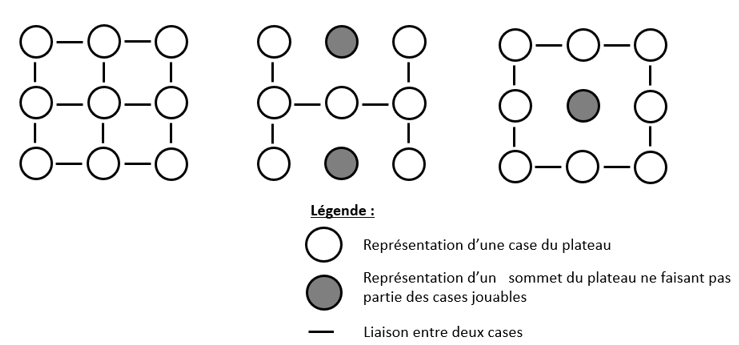
\includegraphics[scale = 0.5]{plateau_carre_tore_h.png}
    \caption{Les plateaux carré, en forme de H et torique}
    \label{fig:plateau_cth}
\end{figure}

\begin{figure}[H]
    \centering
    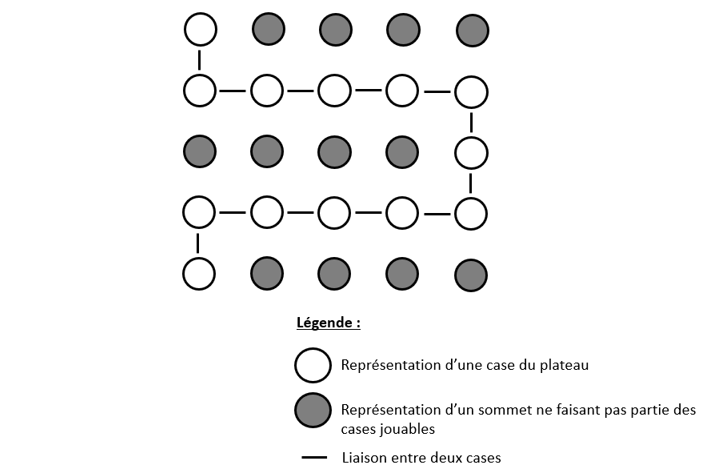
\includegraphics[scale = 0.5]{plateau_serpent.png}
    \caption{Le plateau serpent}
    \label{fig:plateau_s}
\end{figure}

Le plateau de jeu est représenté par une structure \texttt{graph\_t} qui comporte plusieurs champs dont le nombre de sommets, la matrice d'adjacence entre les différents sommets et la matrice indiquant les positions de départ pour chaque joueur. Tout d'abord, nous avons fait en sorte que le sommet en haut à gauche soit le sommet numéroté $0$, le sommet à sa droite est numéroté $1$, et ainsi de suite. La figure \ref{fig:numerote} indique la convention de numérotation des sommets que nous avons choisie.

\begin{figure}[H]
    \centering
    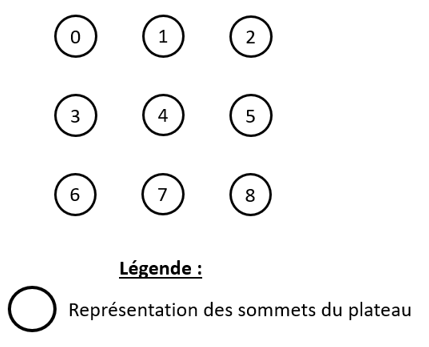
\includegraphics[scale = 0.5]{sommet_plateau.png}
    \caption{Convention de numérotation des sommets choisie}
    \label{fig:numerote}
\end{figure}

Pour implémenter la structure \texttt{graph\_t} qui sert de représentation pour le plateau de jeu, il faut ensuite créer une matrice d'adjacence indiquant la relation entre chaque sommets et la matrice indiquant les positions de départ des joueurs.

Pour remplir la matrice d'adjacence, il nous faut obtenir les différentes relations entre les sommets. Notre convention de numérotation étant toujours ordonnée, nous avons créé une fonction \texttt{get\_direction\_square} prenant les indices de deux sommets, la largeur du plateau et renvoyant le type de connexions entre les deux sommets. De plus, nous avons ajouté des fonctions de prédicat pour chaque type de graphes indiquant si un sommet fait partie des cases jouables ou non du plateau. La fonction \texttt{fill\_graph} utilise ces fonctions afin de remplir correctement la matrice d'adjacence en fonction du type de plateau et de sa taille.

Pour obtenir la matrice des positions de départ nous avons implémenté des fonctions qui regardent la numérotation des sommets et leur attribue le caractère case de départ ou non en fonction. 

Une fois les fonctions d'obtention des différentes matrices créées, nous avons ajouté une fonction générique \texttt{get\_graph} qui retourne une structure \texttt{graph\_t} représentant le plateau en fonction de son type est de sa taille.

En parallèle de la création des différents plateaux, nous avons développé un système d'affichage afin de pouvoir vérifier visuellement les actions des joueurs et leurs répercussions sur le serveur. Pour afficher un plateau, nous parcourons simplement la matrice d'adjacence. 

Les figures \ref{fig:display-c}, \ref{fig:display-t}, \ref{fig:display-h}, \ref{fig:display-s} permettent de se rendre compte de l'affichage mis en place.

\begin{figure}[H]
    \centering
    \begin{subfigure}{.48\textwidth}
        \centering
        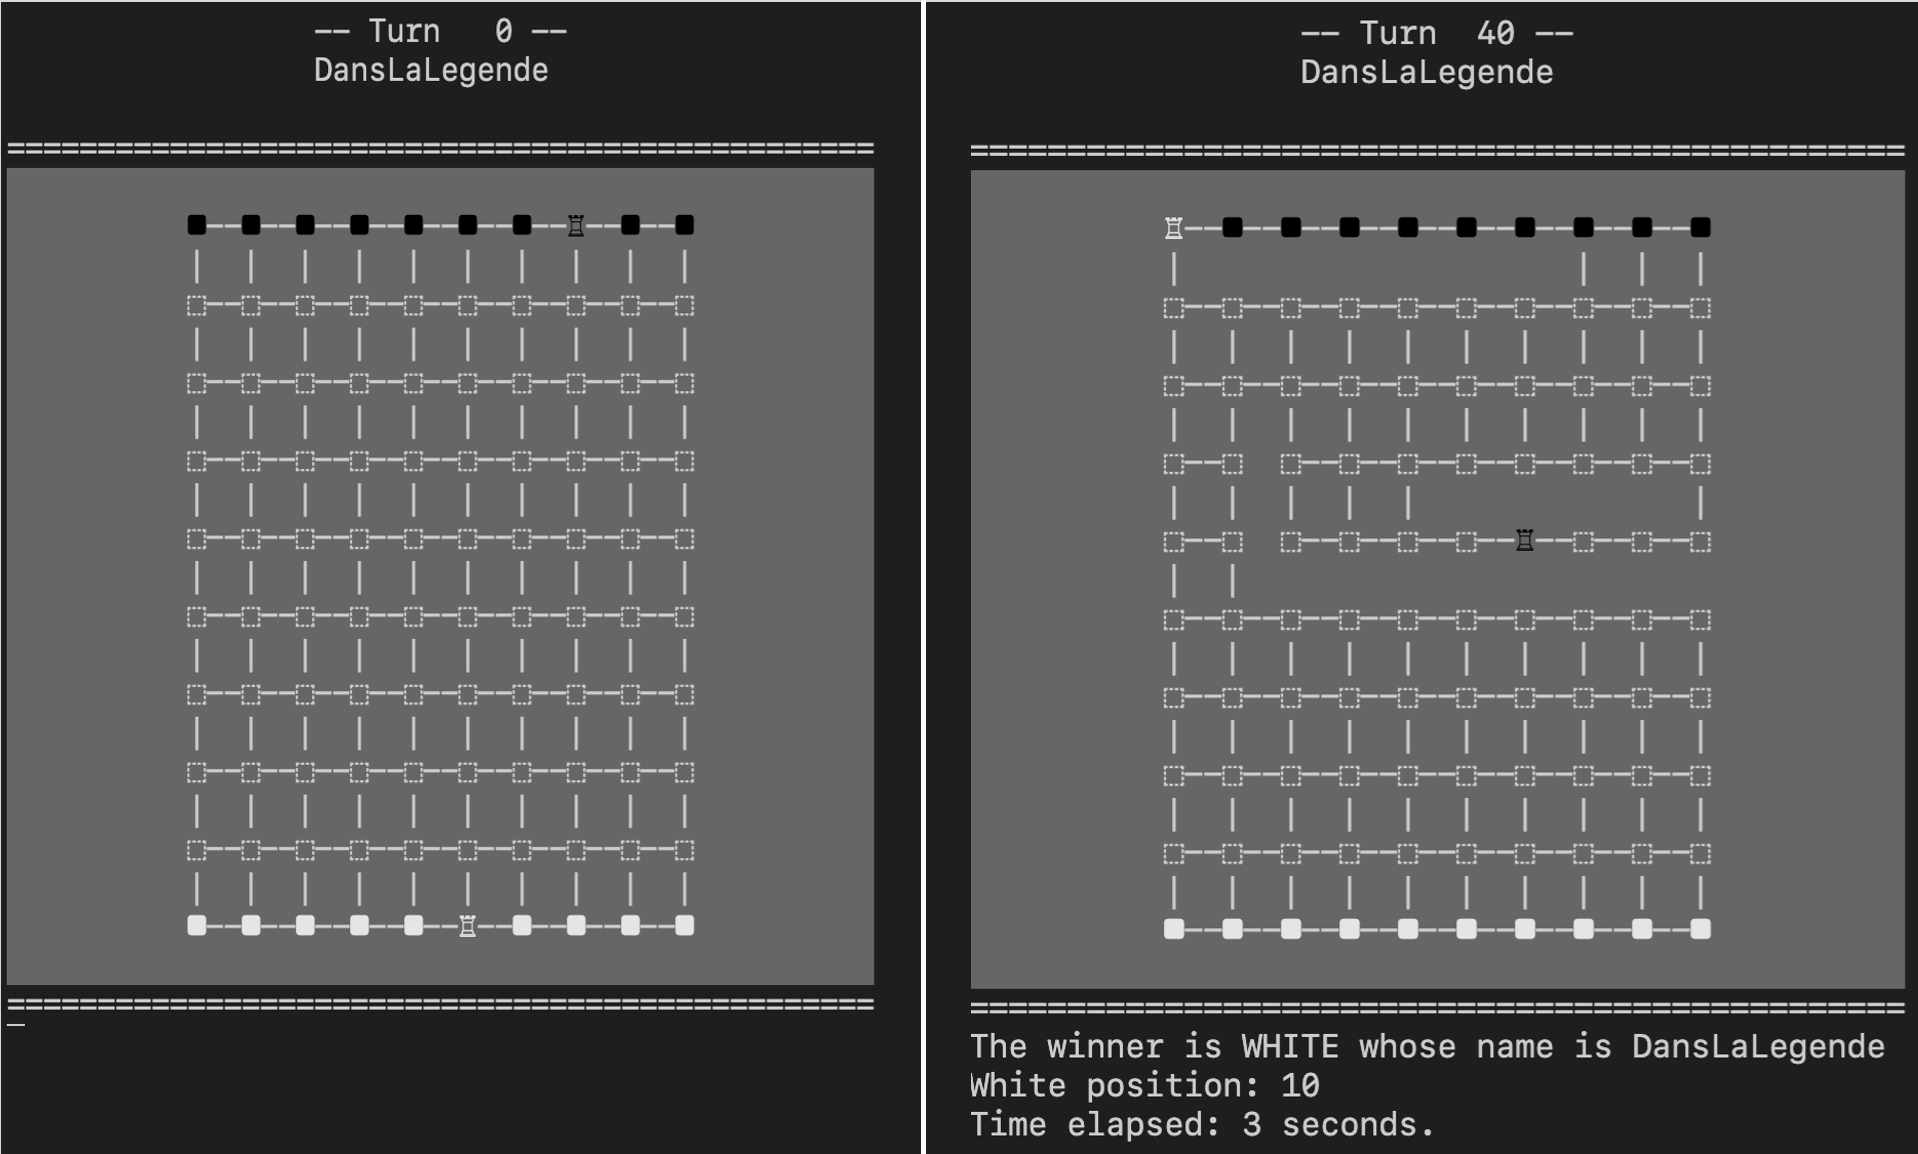
\includegraphics[width=\linewidth, height=.6\linewidth]{display-c.png}
        \caption{Graphe de type carré de 10x10 au premier et dernier tour}
        \label{fig:display-c}
        \hfill
    \end{subfigure}
    \hfill
    \begin{subfigure}{.48\textwidth}
        \centering
        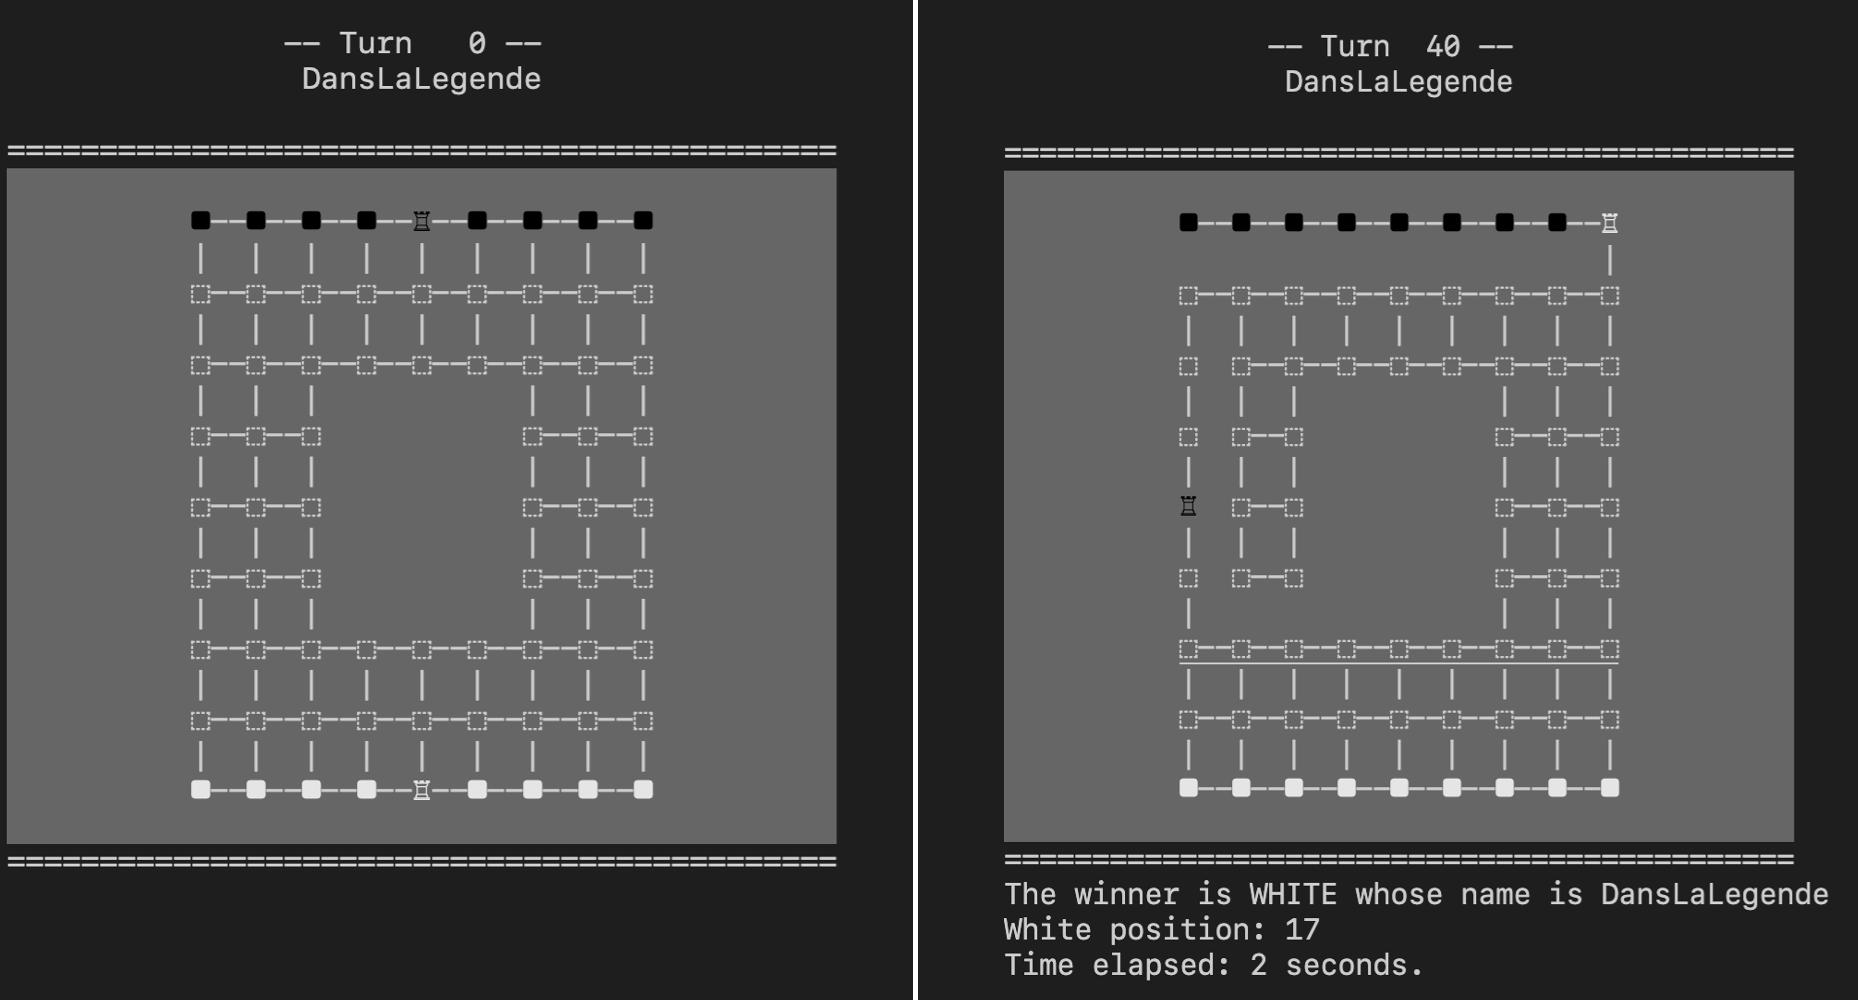
\includegraphics[width=\linewidth, height=.6\linewidth]{display-t.png}
        \caption{Graphe de type torique de 9x9 au premier et dernier tour}
        \label{fig:display-t}
        \hfill
    \end{subfigure}
    \hfill
    \begin{subfigure}{.48\textwidth}
        \centering
        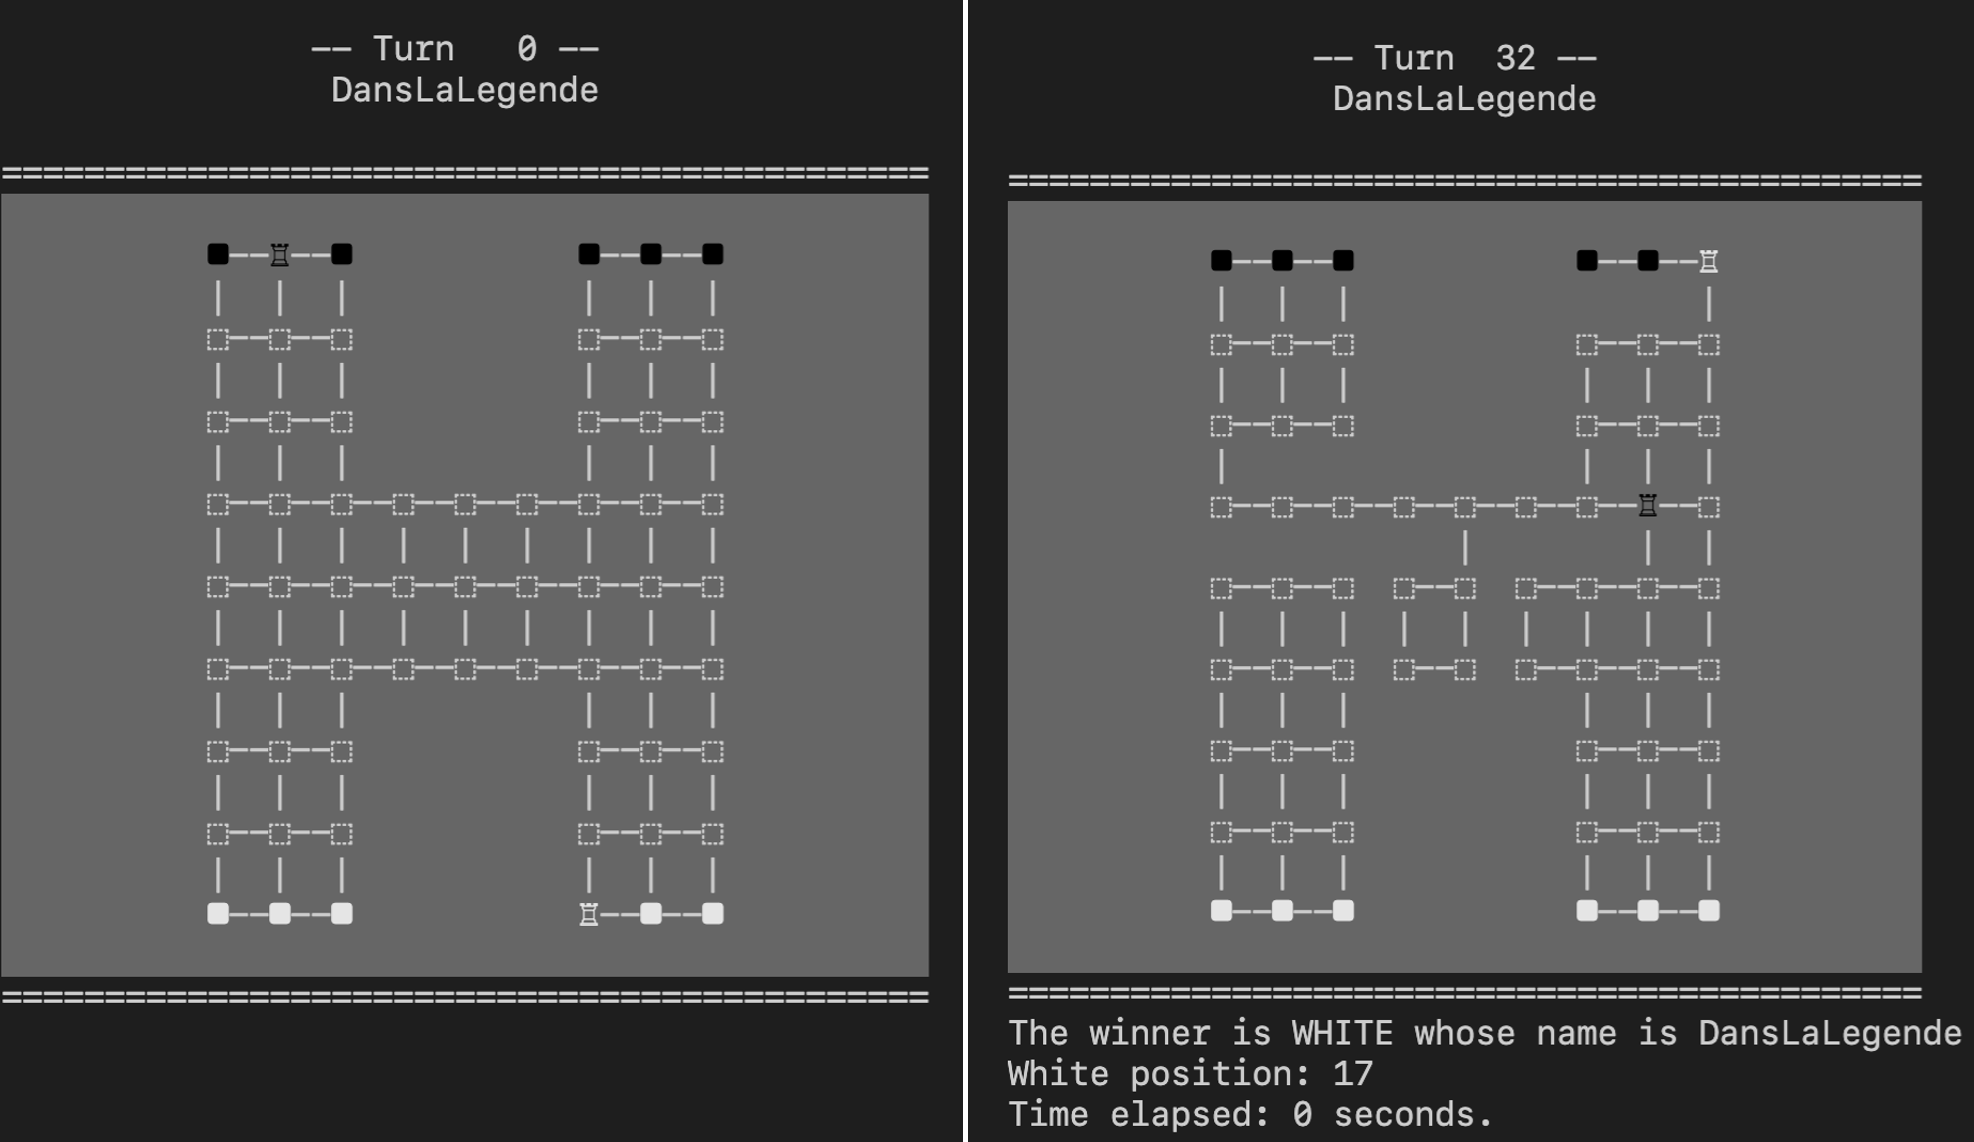
\includegraphics[width=\linewidth, height=.6\linewidth]{display-h.png}
        \caption{Graphe de forme H de 9x9 au premier et dernier tour}
        \label{fig:display-h}
        \hfill
    \end{subfigure}
    \hfill
    \begin{subfigure}{.48\textwidth}
        \centering
        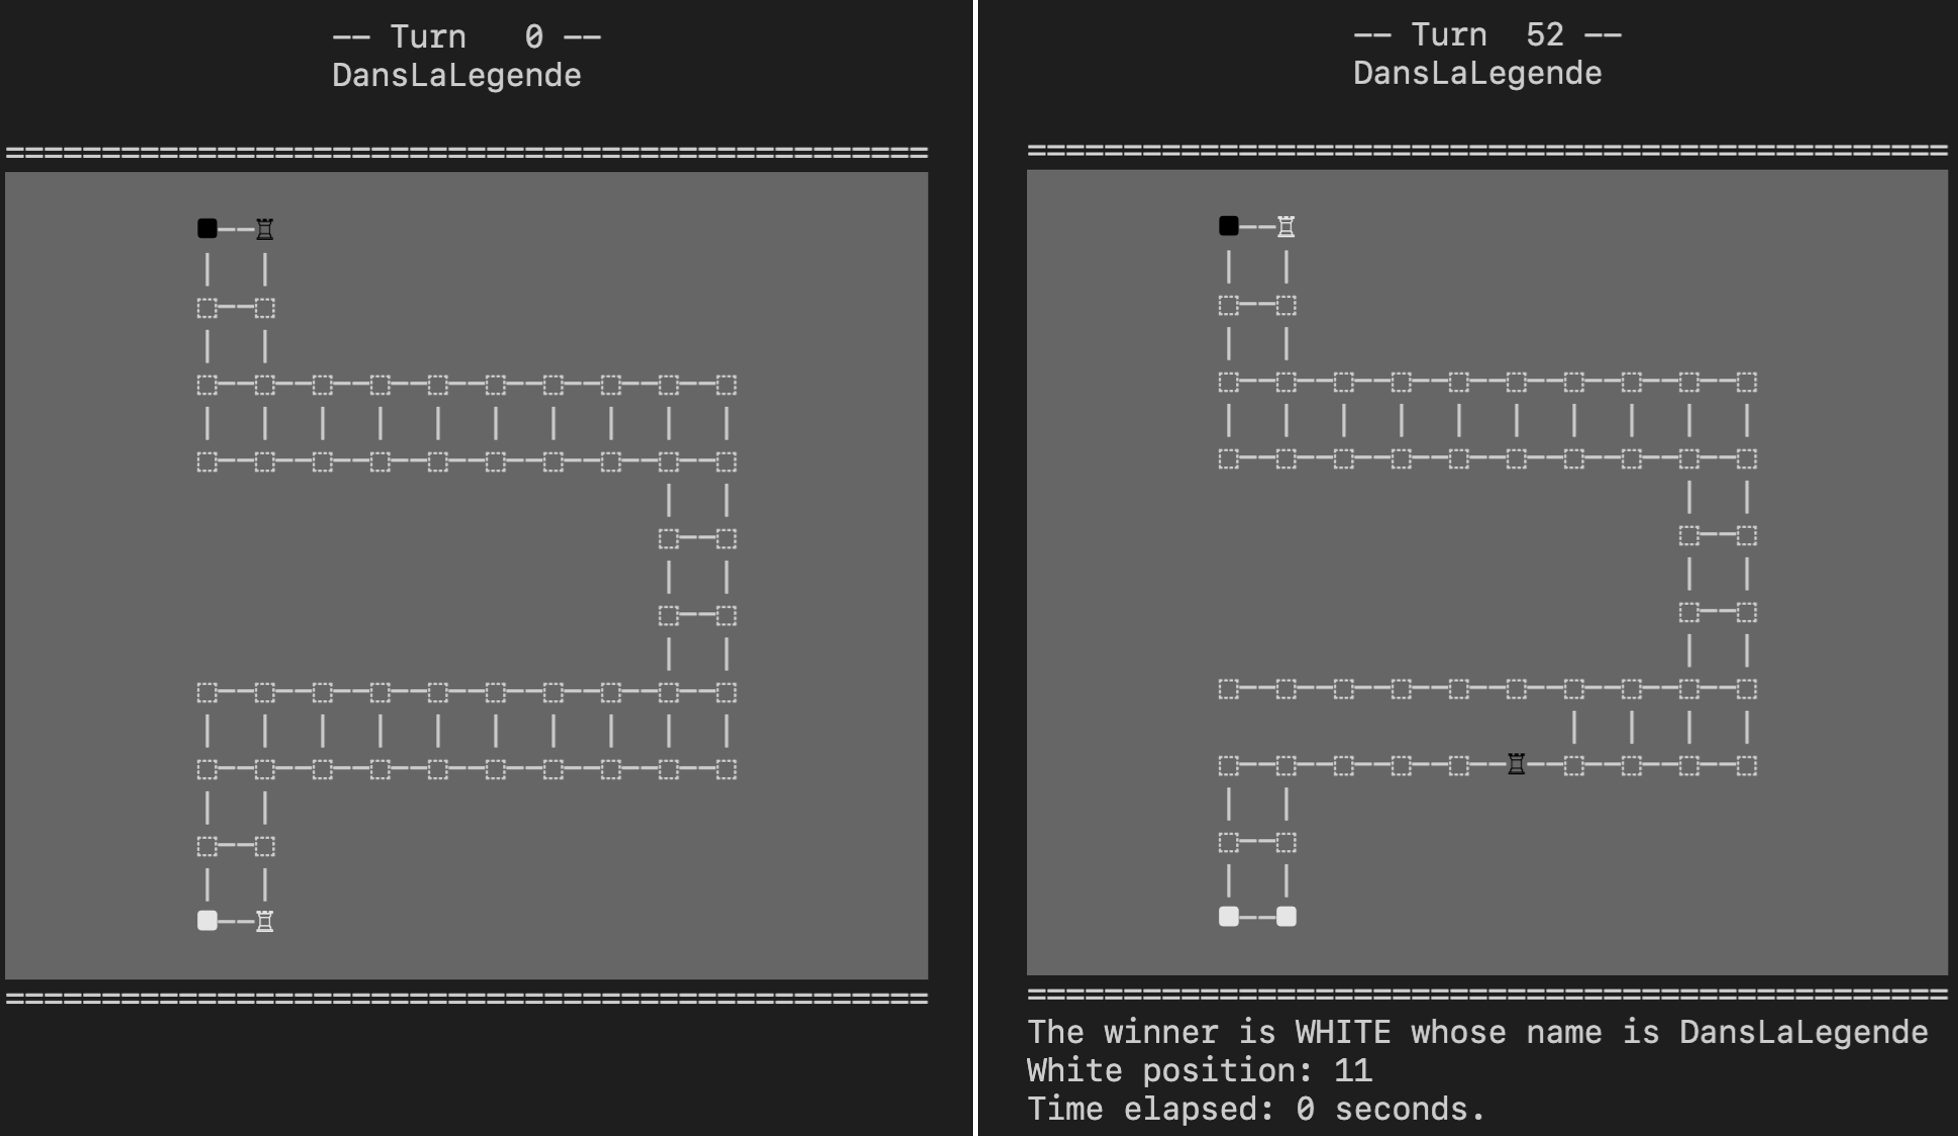
\includegraphics[width=\linewidth, height=.6\linewidth]{display-s.png}
        \caption{Graphe en forme de serpent de 10x10 au premier et dernier tour}
        \label{fig:display-s}
        \hfill
    \end{subfigure}
    \caption{Exemple de l'affichage développé pour les différents types de graphes}
\end{figure}

\subsection{Gestion des joueurs}\label{sec:player-management}

L'une des problématiques est la mise en place d'un échange réglementé entre un serveur et des joueurs. D'un côté, nous pouvons donc trouver un serveur qui permet de faire tourner la boucle de jeu, de vérifier la validité des coups joués et d'indiquer le gagnant. De l'autre, nous trouvons les interfaces joueurs qui implémentent diverses stratégies de jeu et retournent les coups à effectuer. Afin d'obtenir un fonctionnement correct entre les différentes interfaces, nous devons mettre en place un protocole de communication qui permet à toute interface serveur ou joueur de pouvoir communiquer ensemble.

\subsubsection{Présentation du protocole de communication}

Tout d'abord, pour que les interfaces puissent décrypter l'évolution de la partie, nous utilisons deux structures permettant l'échange et la compréhension des différentes informations.

La première structure est la structure \texttt{graph\_t}. Cette dernière permet l'accès aux informations sur le plateau comme le nombre de sommets, le type de connexion entre chaque sommet grâce à une matrice d'adjacence et les sommets de départs. Ainsi elle permet de notifier les modifications effectuées par une interface. 

Une seconde structure est nécessaire aux deux interfaces afin de comprendre les coups joués. Cette structure est la structure \texttt{move\_t}. Elle permet de connaître le type de coup joué que ce soit un déplacement ou la pose d'un mur. Si c'est un déplacement alors le nouveau sommet est indiqué, si c'est un mur alors la structure comprend deux arêtes correspondant aux connexions coupées par le mur. \\

Cependant, la compréhension d'un coup ou du plateau ne suffit pas à la bonne communication entre une interface serveur et une interface joueur, car il faut que le serveur puisse demander et envoyer une information aux clients. C'est pourquoi chaque joueur doit posséder un ensemble de fonctions. Le protocole de communication est donc le suivant :
\begin{itemize}
    \item une fonction \texttt{get\_player\_name} qui ne prend pas de paramètre et retourne le nom du joueur sous la forme d'une chaîne de caractères
    \item une fonction \texttt{initialize} qui initialise un joueur avec un identifiant, le plateau de départ et le nombre de murs autorisés
    \item une fonction \texttt{play} qui prend en argument le coup joué précédemment et retourne le coup suivant joué par le joueur
    \item une fonction \texttt{finalize} qui ne prend pas de paramètre et termine le joueur
\end{itemize}

L'utilisation de fonctions intermédiaires au niveau des joueurs n'est pas interdits, cependant celles-ci ne seront pas accessibles par le serveur. \\

Concernant le plateau de jeu, afin d'éviter une éventuelle triche d'un joueur par modification de la structure \texttt{graph\_t}, le serveur passe une copie de celui-ci aux joueurs et chaque interface devra actualiser son propre plateau et libérer la mémoire de celui-ci à la fin de la partie.

Les joueurs implémentant donc les mêmes fonctions, nous avons utilisé un système de chargement de ceux-ci afin d'éviter les multiples définitions lors de l'édition de liens.

\subsubsection{Chargement dynamique}

Le protocole présenté précédemment présente un inconvénient lorsque l'on souhaite développer plusieurs joueurs. En effet, chaque joueur possède des fonctions avec le même nom et le même prototype et possiblement avec des définitions différentes. Lors de l'édition de liens avec une compilation dite classique, il y aurait un problème de définitions multiples. Afin d'y remédier, le serveur charge les joueurs dynamiquement qui se trouvent être des bibliothèques dynamiques. Ainsi, il ne communiquera qu'avec des instances de joueurs et pas avec le joueur directement. Il peut même appeler le même joueur sous deux instances différentes et le faire jouer contre "lui-même". \\

Les interfaces des joueurs étant individuelles et séparées de l'interface du serveur, il est donc impératif de vérifier chaque coup renvoyé par les clients.

\subsection{Vérification et sanctions} \label{sec:sanctions}

Les règles du jeu Quoridor imposent naturellement des conditions sur les déplacements des joueurs et la pose de leurs murs. Pour résoudre cette problématique, deux fonctions \texttt{can\_player\_move\_to} et \texttt{can\_add\_wall} ont été implémentées, permettant respectivement de valider le déplacement d'un joueur et la pose d'un mur. L'ensemble de ces fonctions agissent conjointement à travers \texttt{is\_move\_legal}, dont la complexité est dominée par celle de \texttt{can\_add\_wall}, qui détermine la légalité d'un coup, en fonction de l'état du plateau, des positions des joueurs et du nombre de murs du joueur actif.

\subsubsection{Vérification d'un déplacement}

La première étape de la vérification de la légalité des coups par le serveur a été de déterminer si un coup de type \texttt{MOVE}, i.e., le déplacement d'un joueur d'une case à une autre, est légal ou non.

Tout d'abord, dans une situation de non face-à-face entre les pions des joueurs, le joueur actif peut bouger vers un sommet \texttt{vertex} dans l'une des quatres directions cardinales connectées à sa position initiale. Ainsi, après vérification de l'existence de \texttt{vertex} dans le graphe grâce à \texttt{is\_vertex\_in\_graph}, et vérification de la disponibilité de ce dernier (c'est-à-dire qu'aucun joueur n'y est positionné) avec \texttt{is\_vertex\_available} (toutes deux de complexité en temps $\mathcal{O}(1)$), la connectivité entre le sommet de la position initiale du joueur et \texttt{vertex} est analysée. Dans le cas où cette connexion existe, alors le déplacement est légal.

Cependant, dans le cas où \texttt{vertex} n'est pas directement accessible, il faut analyser si les deux joueurs sont dans une position de face-à-face (c'est-à-dire que les positions respectives aux deux joueurs sont connectées), ce qui permettrait d'accéder à une position sans connexion directe. Dans cette situation, il faut pouvoir permettre au joueur actif de sauter au-dessus de son adversaire. Cette action permettrait ainsi au joueur actif de passer derrière son adversaire lorsqu'il n'y a pas de mur ou que ce n'est pas le bord du plateau de jeu, sinon sur une case connectée à celle de la position adverse. Afin de réaliser ce type de déplacement, tel qu'illustré par la Figure \ref{fig:correct_move}, trois aspects sont analysés:
\begin{enumerate}
    \item Contrôler si la position adverse est connectée à \texttt{vertex};
    \item Contrôler si la position \texttt{vertex} est derrière l'adversaire par rapport à la position initiale;
    \item Contrôler s'il y a un mur ou le bord du plateau de jeu derrière l'adversaire par rapport à la position initiale.
\end{enumerate}

Ainsi, dans le cas où l'aspect $1$ n'est pas vérifié, alors le déplacement n'est pas possible. D'autre part, si la position adverse est connectée à \texttt{vertex} et que ni l'aspect $2$ ni l'aspect $3$ n'est vérifié, alors le déplacement sera également non légal. La complexité finale de cette fonction est $\mathcal{O}(\log(m^{2}))$, $m$ étant la largeur du graphe/plateau.

Par ailleurs, les placements initiaux des joueurs diffèrent en terme de légalité. Ainsi, cette vérification s'effectue par l'utilisation de \texttt{player\_placement}, déterminant si la position initiale d'un joueur est sur une case lui appartenant.

\subsubsection{Vérification de la pose d'un mur}

La seconde étape de la vérification de la légalité des coups par le serveur a été de déterminer si un coup de type \texttt{WALL}, i.e., la pose d'un mur sur le plateau de jeu, est possible ou non. Le principe de ce contrôle suit un raisonnement inverse à celui de la vérification d'un déplacement. En effet, plutôt que de vérifier si la pose d'un mur est possible, \texttt{can\_add\_wall} va vérifier si cette pose est impossible. Ainsi, dans le cas où cette pose ne valide aucun critère d'impossibilité, alors cette pose est valide. Si la pose est valide alors le mur respecte les propriétés suivantes :
\begin{enumerate}
    \item doit être posé sur le plateau de jeu;
    \item doit être posé entre deux ensembles de positions interconnectées;
    \item doit être posé avec une orientation perpendiculaire à celles des connexions des deux ensembles;
    \item doit être posé entre deux ensembles adjacents de positions;
    \item ne doit pas chevaucher un autre mur;
    \item ne doit pas bloquer l'un des joueurs.
\end{enumerate}

Les difficultés de l'implémentation de cette fonction ont résidé dans la réalisation des critères $5$ et $6$, les autres critères ne correspondant trivialement qu'à de l'analyse des types de connexions ou de leur existence. Ainsi, afin de déterminer si un potentiel mur pourrait chevaucher un mur déjà existant, une fonction \texttt{is\_overlapping\_wall} a été mis en oeuvre, de complexité en temps $\mathcal{O}(\log(m^{2}))$, $m$ étant la largeur du graphe/plateau. Cette dernière exploite l'implémentation d'un type énuméré \texttt{wall\_orientation\_t}, permettant de représenter l'orientation d'une partie d'un mur. Ainsi, lorsqu'un mur est posé, les interconnexions entre ensemble de position d'une structure \texttt{edge\_t} sont modifiées dans la structure du graphe, tel que ces dernières soient
\begin{itemize}
    \item [$\bullet$] \texttt{POINT\_TO\_NORTH} lorsque la seconde partie du mur est en direction du nord;
    \item [$\bullet$] \texttt{POINT\_TO\_SOUTH} lorsque la seconde partie du mur est en direction du sud;
    \item [$\bullet$] \texttt{POINT\_TO\_WEST} lorsque la seconde partie du mur est en direction de l'ouest;
    \item [$\bullet$] \texttt{POINT\_TO\_EAST} lorsque la seconde partie du mur est en direction de l'est.
\end{itemize}
Cette représentation permet ainsi de différencier la présence d'un mur de celle de la non-existence de connexion. Ainsi, l'analyse des types de connexions permet alors de déterminer la présence d'un mur en temps constant.

\begin{figure}[H]
    \centering
    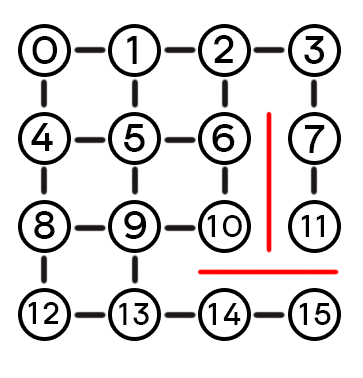
\includegraphics[scale = 0.5]{wall_direction.png}
    \caption{Murs (rouge) placés dans un plateau de largeur $4$}
    \label{fig:wall_direction}
\end{figure}

Par exemple, dans un plateau carré de largeur $4$ avec des murs placés tel qu'illustré par la figure \ref{fig:wall_direction}, alors les connexions dans la matrice représentative du graphe seront changées tel que
\begin{itemize}
    \item [$\bullet$] les connexions entre les vertices $6$ et $7$ soient \texttt{POINT\_TO\_SOUTH};
    \item [$\bullet$] les connexions entre les vertices $10$ et $11$ soient \texttt{POINT\_TO\_NORTH};
    \item [$\bullet$] les connexions entre les vertices $10$ et $14$ soient \texttt{POINT\_TO\_EAST};
    \item [$\bullet$] les connexions entre les vertices $11$ et $15$ soient \texttt{POINT\_TO\_WEST}.
\end{itemize}

La réalisation du critère $6$ utilise un simple parcours en profondeur depuis les positions des joueurs jusqu'à l'ensemble des sommets appartenant à son adversaire. Ainsi, dans le cas où aucun des sommets adverses ne seraient accessibles, alors un des joueurs serait bloqué, et la pose du mur serait alors impossible. Lorsque aucun de ces critères d'invalidités n'est vérifié, alors la pose du mur est valide.

Par ailleurs, la fonction \texttt{can\_add\_wall} ne prend pas en compte le nombre de murs du joueur actif. En effet, cette distinction est faite avec \texttt{is\_move\_legal} qui détermine si le coup d'un joueur est légal ou non, tandis que \texttt{can\_add\_wall} détermine si la pose d'un mur à un certain endroit du plateau est réalisable. La complexité finale de cette fonction et alors dominée par celle du parcours en largeur, i.e., $\mathcal{O}(\log(|V|)(m^{2}+|E|)\cdot\textit{nombre de sommet appartenant à l'adversaire})$, $m$ étant la largeur du graphe/plateau, $|V|$ le nombre de vertices du graphe et $|E|$ le nombre d'arêtes du graphe.

Si une action n'est pas légale alors, elle doit être sanctionnée.

\subsubsection{Sanctions}

Les tours respectifs à chacun des joueurs imposent le retour d'un coup \texttt{move\_t}, permettant de décrire les spécificités du mouvement ou pose de mur du joueur. Cependant, ces coups pourraient ne pas respecter les règles de Quoridor. C'est pour cette raison que lors de chacun des tours des joueurs, leur coup est analysé par \texttt{is\_move\_legal}. 

Dans le cas où le coup est légal, alors le serveur va actualiser le plateau de jeu ainsi que la position des joueurs, respectivement aux conséquences du coup du joueur.

Cependant, dans le cas où le coup réalisé serait illégal, alors le serveur va
\begin{enumerate}
    \item afficher la raison de l'illégalité du coup;
    \item afficher les spécificités du coup réalisé;
    \item attribuer la victoire à l'adversaire;
    \item mettre fin à la partie.
\end{enumerate}


\subsection{Améliorations possibles}

Comme évoqué dans la sous-partie \textit{Présentation de la structure du serveur}, nous avons essayé de rendre générique la notion de serveur à travers trois fonctions principales : \textit{initialize\_server}, \textit{run\_server} et \textit{free\_server}. Nous nous sommes en revanche rendu compte tardivement que nous pouvions améliorer cette vision afin de cacher la définition de la structure d'un serveur. Cela permettrait de créer différents types de serveur. Une idée simple d'un autre serveur aurait été de mettre en place un serveur réalisant un tournoi entre différents joueurs.

Une amélioration de la complexité en temps de l'affichage du plateau a été envisagé afin d'éviter d'appeler constamment la fonction permettant d'afficher dans la sortie standard (actuellement \textit{printf}) ce qui peut être très gourmand en temps. Celle-ci consisterait à remplir une structure de donnée des caractères à afficher afin d'appeler qu'une seule fois cette fonction. Une structure de donnée adéquate serait une file FIFO qui permettrait l'insertion et la récupération d'une information en temps constant.

Une autre amélioration envisagée serait de réaliser une interface pour les fonctions d'affichage et ainsi pouvoir choisir entre plusieurs manières de présenter une rencontre de deux joueurs.

Enfin, la dernière amélioration considérée est celle de rendre non bloquante les fonctions de sanction pour avoir une gestion d'erreur plus souple. C'est-à-dire ne pas forcément quitter le programme dès qu'un joueur réalise un mauvais coup mais simplement de terminer la fonction \textit{run\_server} afin de laisser le programme gérant ce serveur choisir ce qu'il souhaite faire.


\newpage
\section{Joueurs}
Afin de compléter l'architecture serveur-clients, nous avons développé en parallèle du serveur, les différents clients que sont les joueurs. Cette section a pour but d'expliquer le fonctionnement général des joueurs ainsi que les différentes stratégies que nous avons mises en place.

\subsection{Généralités}

Pour implémenter les différents joueurs, le sujet nous imposait l'utilisation du fichier \texttt{player.h} afin de respecter certaines règles et permettre la bonne communication avec le serveur. Comme expliqué en section \ref{sec:player-management}, les joueurs doivent donc, chacun, utiliser quatre fonctions de communications. Cependant, chaque joueur est libre de choisir son implémentation interne.

\noindent Ainsi, nous avons choisi de représenter chaque joueur par une structure \texttt{struct player}, au sein de chaque client, contenant toutes les informations nécessaires à retenir. Cela nous permet d'initialiser une variable globale représentant notre joueur courant. Le joueur joue en travaillant sur sa propre structure, puis communique les résultats au serveur. \\

Le serveur possédant sa propre représentation du graphe d'adjacence, indépendante de celle des joueurs,  un client ne peut pas savoir si les sommets du graphes sont ordonnés ou non. L'accès aux voisins d'une case peut donc devenir compliqué si ces sommets ne sont pas ordonnés. En effet, on ne peut plus uniquement travailler sur les indices des sommets du graphe pour manipuler les cases et leurs voisins. Nous avons donc choisi d'implémenter les graphes de deux manières dans les structures de nos joueurs.
Chaque joueur possède donc, dans sa structure, une structure de graphe \texttt{struct graph\_t} mais également une structure de graphe de corrélation \texttt{struct near\_neighbours}. \\
Cette dernière est une structure contenant quatre indices représentant les indices des sommets adjacents dans les quatre directions d'un sommet donné.
Enfin, à l'aide des fonctions \texttt{get\_correlated\_graph} et \texttt{free\_correlated\_graph} nous pouvons, à partir d'un graphe donné par le serveur, créer un tableau de \texttt{struct near\_neighbours} pour chaque joueur. L'utilisation d'un tableau, permet en effet d'accéder aux voisins d'une case d'indice $x$ en regardant la structure présente à l'indice $x$ du tableau. De plus, la fonction \texttt{free\_corolated\_graph} permet de libérer ce tableau dans la fonction \texttt{finalize} car il a été alloué lors de l'initialisation.\\
Le tableau permet alors de retrouver pour une case donnée (un indice), ses quatre proches voisins dans le graphe en temps constant contrairement à un parcours de toutes les cases du graphe qui serait en temps linéaire. Nous réduisons ainsi la complexité de nombreuses fonctions. Si une case ne possède pas de voisin dans une des directions, alors on lui donne la valeur $m*m$ qui est le nombre maximal de sommets dans le graphe, et donc ne correspond à aucun indice du plateau. \\

\noindent Par exemple, pour un graphe de dimension $m = 3$, le schéma en figure \ref{fig:proches_voisins} illustre la structure en indice $4$ du tableau \texttt{neighbours\_graph} : \\
\indent \texttt{neigbours\_graph[4].north = 1\\ 
        \indent neigbours\_graph[4].south = 7\\
        \indent neigbours\_graph[4].west \ = 3\\
        \indent neigbours\_graph[4].east \ = 9} (pas de voisin dans la direction east) \\
        
\begin{figure}[H]
    \centering
    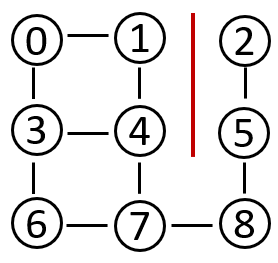
\includegraphics[scale = 0.5]{proches_voisins.png}
    \caption{Schéma des proches voisins}
    \label{fig:proches_voisins}
\end{figure}

Ainsi, lors de l'initialisation d'un client, ce dernier peut, dans la fonction \texttt{initialize} utiliser le graphe donné par le serveur pour créer un tableau des proches voisins de chaque sommet du graphe (indices du tableau). \\
Cette implémentation, nous permet alors d'accéder directement à toutes les case du graphe en naviguant de proches voisins en proches voisins, et évite de devoir parcourir toutes les cases afin de trouver celles qui sont susceptibles de nous intéresser. \\

Nous pouvons donc maintenant, implémenter chaque stratégie de nos différents clients.

\subsection{Stratégie \textit{Random}}

Comme premier joueur, nous avons développé le joueur le plus simple possible. C'est-à-dire un joueur naïf qui n'essaye pas de gagner, mais uniquement de jouer. Ainsi, ce joueur nous a permis de vérifier le bon fonctionnement de notre première version du serveur ainsi que de comprendre les différentes problématiques auxquelles il faut répondre avant de pouvoir implémenter des stratégies plus complexes.

\subsubsection{Implémentation}

Pour implémenter ce client, nous avons, comme pour tous les joueurs, implémenté une structure \texttt{struct player } contenant :
\begin{itemize}
    \item \texttt{graph} un pointeur pointant vers un graph
    \item \texttt{position} un tableau contenant les deux positions des deux joueurs
    \item \texttt{num\_walls} le nombre de murs disponibles pour le joueur
    \item \texttt{id} l'id du joueur \\
\end{itemize}

Ainsi, la fonction \texttt{initialize} permet d'initialiser ces différents champs avec notamment une copie du graphe donnée en paramètre par le serveur. \\

Lors de l'appel à la fonction \texttt{play}, notre joueur regarde s'il est déjà placé sur le plateau de jeu en temps constant. Ceci est possible à l'aide d'une astuce lors de l'initialisation : la position est initialisée à une valeur supérieure au nombre de sommet présent représentant le plateau de jeu. S'il n'est pas déjà placé, alors il retourne une action de type MOVE correspondant au placement aléatoire parmi les cases disponibles sur la ligne de départ au travers de la fonction \texttt{get\_first\_move}. Sinon, il fait appel à l'algorithme \texttt{get\_new\_move} qui regarde les cases accessibles parmi toutes les cases du jeu, les retient temporairement afin d'en choisir une aléatoirement et de retourner l'action de \textit{déplacement} correspondant. \\

\noindent Pour cela, nous faisons appel à une procédure \texttt{get\_available\_positions} qui parcourt toutes les cases du graphe et complète un tableau passé en paramètre. Ainsi, il ne reste plus qu'à créer correctement un \textit{move} avec une des positions possibles choisie de manière aléatoire. \\

\noindent La fonction \texttt{play} d'un joueur doit aussi réaliser la mise à jour des éléments du joueur par rapport à son action à lui, mais également à celle du joueur adverse. Plus spécifiquement, il s'agit dans notre cas de réactualiser le graphe de notre joueur. Après réception d'une action adverse, nous mettons donc à jour le graphe du joueur à l'aide de la fonction \texttt{update}. Selon le type d'action, cela peu correspondre à mettre à jour la nouvelle position du joueur ou bien à l'ajout d'un nouveau mur. Nous utilisons également cette fonction avant de retourner notre propre \textit{move}.

\subsubsection{Avantages, inconvénients et améliorations possibles}

L'avantage de ce joueur est qu'il est très simple à mettre en place. Il nous a donc permis de coder un client très rapidement afin de tester notre serveur. Nous avons ainsi rapidement pu lancer des parties en faisant jouer ce client pour chacun des joueurs. \\

Cependant, comme il se déplace de façon aléatoire, il est possible qu'il aille dans la mauvaise direction, jusqu'à revenir sur la ligne de départ. Également, il ne pose aucun mur, donc il n'empêche absolument pas le joueur adverse d'aller en ligne droite vers une position gagnante. \\

Afin d'améliorer ce joueur, tout en gardant le côté aléatoire, il serait judicieux de jouer intelligemment, et de choisir aléatoirement parmi une liste de coup qui restent avantageux pour le joueur. Ainsi le joueur choisirait aléatoirement de bloquer d'une façon ou d'une autre le joueur adverse, ou de se déplacer à tel ou tel endroit afin de progresser vers la ligne d'arrivée.

\subsection{Stratégie \textit{Forrest Gump}}
\label{sec:ForrestGump}

L'un de nos clients implémenté est nommé Forrest Gump. En effet, à la manière du célèbre personnage, ce client ne fait que courir le plus vite possible vers la ligne d'arrivée.

\subsubsection{Implémentation}

Pour implémenter ce client, nous avons, comme pour tous les joueurs, implémenté une structure \texttt{struct player } contenant :
\begin{itemize}
    \item \texttt{graph} un pointeur pointant vers un graph
    \item \texttt{neighbours\_graph} un tableau de corrélation (proches voisins)
    \item \texttt{position} un tableau contenant les deux positions des deux joueurs
    \item \texttt{num\_walls} le nombre de murs disponibles pour le joueur
    \item \texttt{best\_direction} la direction du joueur, Sud s'il commence au Nord et inversement
    \item \texttt{id} l'id du joueur
\end{itemize}

Comme pour le joueur random, la fonction \texttt{initialize} permet l'initialisation de ces champs utilisant les fonctions de copie du graphe envoyé par le serveur, et de la fonction \texttt{get\_correlated\_graph} pour la construction du graphe de corrélation. \\

\noindent Cette stratégie se basant sur celle du joueur \textit{Random}, la fonction \texttt{play} reprend le principe de :
\begin{enumerate}
    \item Mise à jour du joueur avec l'action du joueur adverse;
    \item S'il s'agit du premier tour du joueur, choisir une position de départ, sinon choisir un mouvement à réaliser;
    \item Mise à jour du joueur avec sa nouvelle action;
    \item Retourner cette action.
\end{enumerate}

La différence avec le joueur se fait au niveau du choix de mouvement lors de l'étape $3$ à l'aide de la fonction \texttt{get\_new\_move}.
Dans ce joueur, cette fonction utilise l'implémentation du tableau des corrélations pour calculer en temps constant et tester chacune des douze cases accessibles depuis la position du joueur.
En effet, comme le montre le schéma de la figure \ref{fig:douzecases}, un joueur peut possiblement accéder à douze cases autour de lui en fonction des positions des murs et de l'autre joueur. Sur le schéma sont représentées les douze cases accessibles numérotées par ordre de priorité.

\begin{figure}[H]
    \centering
    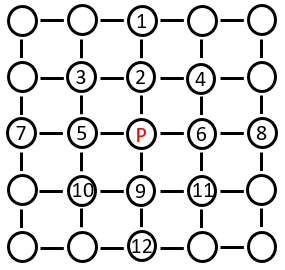
\includegraphics[scale = 0.4]{douzecases.png}
    \caption{Cases accessibles par ordre de priorité}
    \label{fig:douzecases}
\end{figure}

Ainsi, la fonction \texttt{get\_new\_move} teste ces douze cases selon un ordre de priorité et retourne la première case formant un déplacement valide. \\
Les cases sont en effet testées selon un ordre de priorité comme le montre le schéma en figure \ref{fig:douzecases}.
La première case testée est celle la plus proche de la ligne d'arrivée, donc deux cases plus loin que le joueur dans la direction \texttt{best\_direction}. Ensuite, on teste la case collée à celle du joueur dans cette direction. Puis les deux cases en diagonal vers l'avant sont testées, le joueur y a accès s'il peut sauter par-dessus le joueur adverse et qu'il y a un mur derrière, alors il rebondit et accède à l'une de ces deux cases si elles sont disponibles. La fonction s'arrête donc dès qu'une case accessible est trouvée, pour éviter de faire des tests inutiles sur les cases suivantes.

La figure \ref{fig:acces} illustre les possibilités d'accès aux cases 1 à 8. On obtient facilement les cases 9 à 12 par symétrie.

\begin{figure}[H]
    \centering
    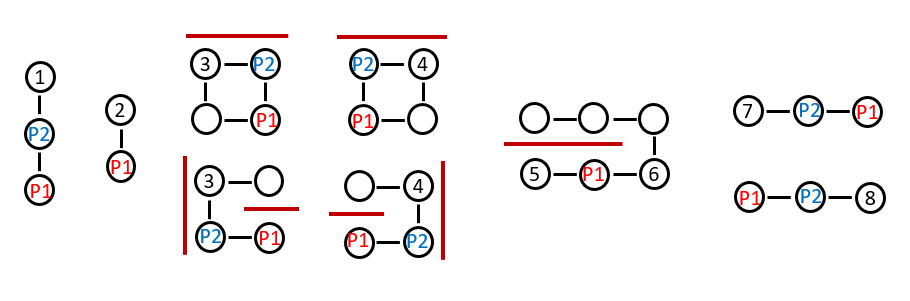
\includegraphics[scale = 0.4]{acces.png}
    \caption{Accès aux différentes positions}
    \label{fig:acces}
\end{figure}

Pour obtenir les indices des douze cases à tester, nous appelons la fonction \texttt{get\_vertices\_to\_test} qui utilise le tableau des corrélations pour trouver les proches voisins par rapport à la position du joueur. Ainsi, en fonction de la \texttt{best\_direction}, du joueur, elle complète un tableau passé en paramètre avec les cases à tester dans l'ordre de priorité. \\

\subsubsection{Avantages, inconvénients et améliorations possibles}

Ce client, comme son nom l'indique, est donc très rapide face à un joueur qui n'essaye pas de le bloquer. \\

Cependant, il ne prend jamais en compte l'autre joueur, à part lui sauter par-dessus, il n'essaye jamais de le bloquer. Ainsi, ce client est plutôt naïf, car il ne cherche pas à bloquer son adversaire, cependant face à un joueur adverse naïf également, il sera très rapide et gagnera la plupart des parties. \\

Pour améliorer ce client, il serait donc judicieux de prendre en compte la position de l'autre joueur, pour par exemple essayer de l'amener vers nous avec des murs et ensuite l'utiliser pour sauter par-dessus. En effet, pour l'instant cela n'est possible si les deux joueurs se retrouvent "par hasard" l'un en face de l'autre. Ainsi, ce client serait plus performant, si en plus de courir tout droit, il posait des murs judicieusement pour contrôler la position de l'autre joueur.

\subsection{Stratégie spécifique à un type de joueur : \textit{AntiBolt}}

\subsubsection{Théorie}

Une stratégie simple pour gagner une partie est tout simplement d'aller tout droit quand cela est possible pour atteindre une case gagnante. C'est l'une des premières stratégies mise au point par les autres équipes de projet. Nous avons alors décidé de créer un joueur capable de la contrer. Pour cela, notre stratégie \textit{AntiBolt} doit empêcher le joueur adverse d'aller en ligne droite s'il peut gagner. L'idée est de regarder si le joueur adverse gagne en allant tout droit. Si c'est le cas, \textit{AntiBolt} pose un mur devant la case d'arrivée. Cette vérification se fait à chaque tour. Ainsi, si au tour suivant, le joueur adverse peut de nouveau gagner en allant tout droit, alors notre joueur pose à nouveau un mur si cela est possible. Si aucun mur n'est à placer, notre stratégie privilégie le déplacement en ligne droite vers les cases d'arrivées, si cela n'est pas possible alors elle choisit un autre déplacement, selon la priorité que nous lui avons donnée.

\subsubsection{Implémentation}

Pour implémenter cette stratégie, nous avons choisi de créer un joueur nommé \textit{AntiBolt} qui reprend l'implémentation du joueur \textit{ForrestGump} précédemment présenté auquel nous avons ajouté une fonction \texttt{get\_wall} qui renvoie une action indiquant s'il doit poser un mur ou non. Si oui, cette action correspond au mur à poser. Le mur est ainsi placé de manière à couper l'arête permettant d'accéder à la case d'arrivée. 

La fonction \texttt{get\_wall} consiste à regarder dans un premier temps, au travers de la fonction auxiliaire \texttt{can\_fast\_forward}, si le joueur adverse peut gagner en allant en ligne droite (complexité en temps  de l'ordre au plus du nombre de sommet du graphe). Cette fonction renvoie l'index de la case d'arrivée si le joueur peut aller en ligne droite, sans prendre en compte la présence de murs, sinon elle retourne un index de sommet invalide.
Dans le cas ou l'index renvoyé par \texttt{can\_fast\_forward} est valide, \texttt{get\_wall} créée un mur coupant l'arête permettant l'accès à la case d'arrivée et vérifie s'il peut être mis à cet endroit.

En conclusion, si le joueur adverse ne peut pas gagner en allant en ligne droite ou si notre joueur ne peut pas poser de mur alors le \texttt{move} renvoyé par \texttt{get\_wall} est de type \texttt{NO\_TYPE} indiquant ainsi que le joueur doit se déplacer au lieu de poser un mur. Le déplacement est quant à lui, géré de manière identique à celle du joueur \texttt{ForrestGump}. 

\subsubsection{Améliorations possibles}

En confrontant le joueur \textit{AntiBolt} à d'autres joueurs, nous nous sommes rendu compte que sa stratégie de déplacement n'est pas optimale dans le cas où le joueur adverse pose lui aussi des murs. De plus, dans certains cas notre joueur en posant un mur pour bloquer l'autre joueur peut aussi se bloquer. 

\subsection{Stratégie spécifique améliorée : \textit{IntelligentAntiBolt}}

\subsubsection{Principe}

Cette stratégie consiste à améliorer le mode de déplacement de la stratégie \texttt{AntiBolt}. Nous avons choisi d'utiliser l'algorithme de \textit{Dijsktra} permettant d'obtenir le plus court chemin pour atteindre une case d'arrivée. Cette recherche se fait en un temps de l'ordre de $\mathcal{O}(|E|+|V|log(|V|))$ où $|E|$ est le nombre d'arêtes et $|V|$ le nombre de sommets. Le choix entre l'action de poser un mur ou de se déplacer se base sur la même stratégie que pour le joueur \texttt{AntiBolt}. Afin de pouvoir utiliser cette manière de rechercher un plus court chemin, nous avons commencé par écrire une fonction \texttt{dijsktra} générique, prenant un graphe, la position du joueur source ainsi que la position du joueur adverse et les cases d'arrivée. De cette manière, tout type de joueur ou de serveur peut utiliser cet algorithme.

\subsubsection{Améliorations possibles}

Une première amélioration de notre joueur serait d'améliorer le choix de pose de mur, car actuellement, poser un mur juste devant les destinations gagnantes peut ne pas rallonger suffisamment la distance du joueur adverse.

Une autre amélioration possible impliquerait une amélioration de notre algorithme \textit{Dijsktra} afin de ne pas recalculer le plus court chemin à chaque tour, mais seulement si un mur a été posé ou si un saut devient possible (le joueur ennemi est à côté de notre joueur). Une solution serait de retourner une structure \texttt{dijsktra} contenant les informations nécessaires afin de connaître en temps constant les sommets appartenant au chemin le plus court.


\subsection{Stratégie Minimax}

\subsubsection{Théorie}

L’algorithme de recherche Minimax \cite{Minimax} représente le pilier de méthodes de recherche plus complexes tel que l’élagage Alpha-Beta. Cette recherche récursive suppose que l’adversaire jouera de façon optimale, c’est-à-dire qu’il cherchera à effectuer le meilleur coup possible dans toutes les situations. Cette hypothèse  permet ainsi de décider le coup à effectuer, amenant à minimiser la perte de la pire éventualité qui pourrait survenir à la suite d’un nœud donné dans un arbre de jeu. 

Selon cette stratégie, les joueurs sont divisés en deux types. D'une part, le joueur maximisant, cherchant à atteindre l’utilité maximale possible et qui jouera le coup à l'origine de la branche permettant d’atteindre cette utilité. D’autre part, le joueur minimisant, cherchant à minimiser l’utilité du joueur maximisant. Il s’agit d’un point d’information crucial permettant de déterminer quelle branche le joueur maximisant prendra. La valeur minimax de tout nœud de l'arborescence de jeu peut-être calculée de manière récursive, tel que

\begin{equation}
    \text{ValeurMinimax(n\oe ud)}=\left\{
    \begin{matrix}
        \text{Utilit\'e(n\oe ud)} & \text{si n\oe ud terminal}\\ 
        \underset{v \in \text{successeurs(n\oe ud)}}{\max}\left ( \text{ValeurMinimax(v)} \right ) & \text{si joueur maximisant}\\ 
        \underset{v \in \text{successeurs(n\oe ud)}}{\min}\left ( \text{ValeurMinimax(v)} \right ) & \text{si joueur minimisant}
    \end{matrix}
    \right. .
\end{equation}

On notera la nature récursive de la fonction, ainsi que la symétrie du comportement des joueurs maximisant et minimisant. Ainsi, cette stratégie repose sur la construction d'un arbre des possibilités à partir de l'ensemble des coups légaux possibles à partir d'un état du jeu. L'arbre de jeu est alors construit récursivement, de telle sorte qu'un noeud et ses successeurs alternent entre le joueur maximisant et le joueur minimisant. Dès lors que l'arbre est de la profondeur de recherche désirée ou que l’arborescence ne peut pas continuer à partir de ce nœud (victoire de l'un des joueurs dans le cadre du jeu Quoridor), le n\oe ud est alors terminal et l’utilité du plateau de jeu est déterminée à l’aide d’une fonction d'évaluation rendant compte de l’état actuel du plateau pour un joueur donné. Ainsi, chaque utilité “remonte” l'arbre récursivement construit, permettant de déterminer le coup à effectuer.

\subsubsection{L'élagage Alpha-Beta}

L’élagage Alpha-Beta \cite{alphaBeta} est une amélioration par rapport à la recherche Minimax. Il repose sur le fait qu’il est possible de calculer la décision Minimax exacte sans avoir à élargir la portée de tous les nœuds de l’arborescence du jeu, car on peut souvent savoir à l’avance que certaines branches ne peuvent pas mener à un nœud avec une utilité optimale. 

Afin de réaliser cet élagage, il suffit de sauvegarder les valeurs extrêmes $\alpha$ et $\beta$ d'utilité trouvées au cours de l'évaluation récursive, tel que

\begin{equation}
    \left\{\begin{matrix}
        \alpha & = & \text{La plus grande valeur d'utilit\'e trouv\'ee jusqu'ici}\\ 
        \beta & = & \text{La plus petite valeur d'utilit\'e trouv\'ee jusqu'ici}& 
    \end{matrix}\right..
\end{equation}

Pour chaque nœud exploré lors de la recherche à travers l’arbre de jeu, on compare son utilité à $\alpha$ et $\beta$ pour savoir si l’on peut élaguer des branches. Il faut ainsi mettre à jour les valeurs de $\alpha$ et $\beta$ avec les meilleures valeurs trouvées jusqu’alors durant la recherche dans l’arborescence de jeu.

\subsubsection{Implémentation}

Une fois la théorie de la recherche Minimax comprise, le prochain obstacle est de pouvoir la mettre en œuvre. 

Tout d'abord, la structure du joueur \texttt{struct player} utilisée afin de représenter le joueur est simple et ne stocke que les informations essentielles à la sauvegarde de l'état d'une partie. Ainsi, la structure de l'implémentation de la stratégie Minimax s'articule trivialement avec
\begin{itemize}
    \item [$\bullet$] un pointeur \texttt{graph} vers une structure \texttt{graph\_t}, décrivant l'état du plateau par son graphe;
    \item [$\bullet$] un pointeur \texttt{neighbours\_graph} vers une structure \texttt{near\_neighbours}, permettant d'obtenir les voisins directs aux sommets dans le graphe;
    \item [$\bullet$] un tableau \texttt{position} de \texttt{size\_t}, permettant de stocker les positions respectives de chacun des joueurs;
    \item [$\bullet$] un \texttt{size\_t num\_walls}, permettant de faire un suivi du nombre de murs restant;
    \item [$\bullet$] le \texttt{id} du joueur, décrivant sa couleur \texttt{enum color\_t}.
\end{itemize}

L'algorithme de la stratégie Minimax en lui-même est trivial. Cependant, son implémentation a tout d'abord nécessité l'implémentation du type de données de liste \texttt{struct list}, afin d'avoir une structure de donnée permettant de stocker, ajouter et accéder à l'ensemble des coups légaux d'un joueur. Cette implémentation s'est faite de façon dynamique, de telle sorte que le tableau stockant les adresses des éléments de la liste double sa capacité \texttt{capacity} lorsque le tableau est plein, i.e. lorsque sa taille \texttt{size} est la même que sa capacité. Un tel choix a été effectué dans le but d'avoir une complexité constante $\mathcal{O}(1)$ pour les opérations d'ajout, d'accession et de changement d'élément, et pour celle permettant d'obtenir le nombre d'éléments stockés par la liste.

D'autre part, la fonction d'évaluation \texttt{heuristic\_evaluation} (de complexité $\mathcal{O}(\log(|V|)(m^{2}+|E|)\cdot\textit{nombre de vertices appartenant à l'adversaire})$, $m$ étant la largeur du graphe/plateau, $|V|$ le nombre de sommets du graphe et $|E|$ le nombre d'arêtes du graphe) d'un état du plateau de jeu consiste à comparer les distances respectives au joueur actif et à son adversaire pour gagner. Ainsi, la distance du joueur actif pour gagner est soustraite à la distance de son adversaire pour gagner, permettant d'avoir une valeur d'utilité positive lorsque le joueur actif est plus proche de gagner que son adversaire. Ce calcul de distance est assuré par \texttt{get\_minimal\_distance\_to\_opponent\_area}, et utilise un algorithme de parcours en largeur permettant de déterminer la distance minimale entre la position d'un joueur et les sommets appartenant au joueur adverse. La complexité en temps de ce calcul est alors celle du parcours en largeur, multipliée par le nombre de sommets appartenant au joueur adverse, tout en tenant compte du temps de recherche dans un AVL de la librairie GSL. La mise en \oe uvre de cet algorithme de parcours en largeur s'est servie du type de donnée de file \texttt{struct queue}, implémentée naturellement à l'aide d'une liste chaînée, ainsi que de pointeurs vers la tête et la queue de cette dernière, permettant ainsi d'avoir des complexités constantes dans les opérations utilisées, i.e., celles d'enfilement et défilement. Par ailleurs, il est à noter que dans le cas d'une victoire du joueur actif (resp. son adversaire), une valeur représentant une utilité infinie (resp. $-\infty$) est retournée, afin de permettre un meilleur élagage.

Le temps de calcul étant directement lié à la profondeur de l'arbre et à son nombre d'embranchement, une contrepartie a été de réduire le nombre de coups possibles pour le joueur actif. En effet, le nombre moyen de coups possibles dans une partie de Quoridor étant de $60$, la décision faite a été d'éliminer en grande partie les coups consistants à poser des murs. Les seuls coups de pose de mur utilisés dans l'arborescence de l'arbre sont alors ceux comportant un sommet qui correspond à la position du joueur adverse. Cet élagage de coups a été réalisé grâce à la structure \texttt{near\_neighbours}, permettant d'accéder aux voisins directs de la position du joueur adverse en temps constant. Cette modification a ainsi permis de réduire le nombre moyen de coups d'un facteur $10$, permettant alors notamment d'effectuer une recherche de profondeur plus élevée tout en réduisant le temps de jeu. La complexité de l'implémentation de l'algorithme Minimax avec Alpha-Beta Pruning est donc $\mathcal{O}(6^{depth})$ dans le pire des cas (pas d'élagage).

Finalement, la fonction \texttt{get\_new\_move} permet de déterminer le coup à jouer, en itérant parmi tous les coups légaux  élagués du joueur et en lui appliquant l'algorithme Minimax avec élagage Alpha-Beta, afin de lui attribuer une valeur d'utilité. Le coup choisi est alors celui avec la plus grande utilité. Il est à noter qu'un algorithme similaire a aussi été implémenté, Negamax, qui est strictement équivalent à l'algorithme Minimax, la différence résidant dans la taille de leur algorithme respectif. Cela a permis d'avoir une meilleure compréhension de la théorie sous-jacente avant d'effectuer des simplifications d'écriture.

\subsubsection{Améliorations possibles}

Ce projet étant réalisé en temps limité, certaines améliorations - n'ayant pas été réalisées afin d'avoir une sécurité face à cette limite temporelle - auraient pu être réalisées.

La stratégie Minimax ne représente que le commencement d'algorithmes de décisions plus complexes. Dans le cadre de ce projet, l'élagage Alpha-Beta a été réalisé afin de réduire la complexité temporelle de la stratégie Minimax. Cependant, d'autres améliorations sont encore possibles.

En effet, l'une des faiblesses de l'utilisation de l'algorithme de Minimax repose dans sa complexité temporelle exponentielle. Ainsi, il devient alors difficile de réaliser des arborescences de jeu de profondeur élevée, d'autant plus que dans le cadre du \textit{Ladder}, l'ordre de grandeur du temps de décision de chaque coup est de $0.2s$.

Ainsi, afin de réduire la complexité temporelle, une première amélioration aurait pu être d'augmenter la complexité spatiale. Une telle amélioration aurait alors pu être effectuée à travers l'utilisation d'une table de transposition, implémentée avec une table de hashage, ce qui aurait alors permis de ne pas recalculer une branche et ses successeurs plusieurs fois. Une telle modification aurait aussi permis d'effectuer un ordonnancement des coups en fonction de leur capacité à pouvoir élaguer l'arbre de jeu à travers l'élagage Alpha-Beta.

Suite à une telle amélioration, une implémentation simple possible aurait pu être de l'utiliser avec un algorithme MTD-f (Memory-enchanced Test Driver with node n and value f). Cette modification aurait ainsi permis de réduire itérativement la fenêtre de recherche de l'élagage Alpha-Beta précédemment développé et ainsi induire plus de coupure de l'arborescence. Cette amélioration aurait alors été couplée avec une recherche itérative d'approfondissement en profondeur, augmentant de manière itérative la profondeur de recherche.


\newpage
\section{Architecture du projet}
Cette section a pour but de présenter l'ordonnancement des différents fichiers selon leur thématique ainsi que les dépendances qui y sont liées.

\subsection{Ordonnancement des fichiers}
L'organisation des différents fichiers sources du répertoire s'est réalisée selon un regroupement par thématique. En effet, nous avons vite remarqué qu'un nombre important de fichiers pourraient être amenés à être présent dans le répertoire source. Afin de ne pas se perdre, nous avons pris la décision de regrouper certains fichiers sources dans les thématiques suivantes : joueurs, tests, en-tête, serveur et enfin les fichiers communs au serveur et aux joueurs. Cette décision fut aussi prise afin de pouvoir compiler les fichiers binaires correctement avec les bonnes options de compilations en particulier pour les objets ou les tests.

Les fichiers sources correspondant aux implémentations des joueurs se trouvent dans un sous dossier \textit{player}, ceux des tests dans le sous dossier \textit{tests}, les fichiers en-tête étant dans le sous répertoire \textit{include} et les fichiers en commun dans un sous dossier \textit{common}. Les fichiers constituant le serveur sont, quant à eux, à la racine. 

L'ordonnancement des fichiers est représenté par l'arborescence décrite par la figure \ref{fig:files-tree-structure} fournie en Annexe.

\subsection{Dépendances entre les différents fichiers}
Nous pouvons voir à l'aide de la figure \ref{fig:dependency-graph} que notre projet se base sur le fichier \textit{header move} et sur le fichier source \textit{utils}. En effet, ce sont les fichiers principaux du projet. Le premier permet de définir ce qu'est un move tandis que le deuxième permet d'avoir accès aux fonctions de vérifications, de sanctions mais également de copie, de libération ou d'accès à un élément de la matrice d'adjacence.

\begin{figure}[H]
    \centering
    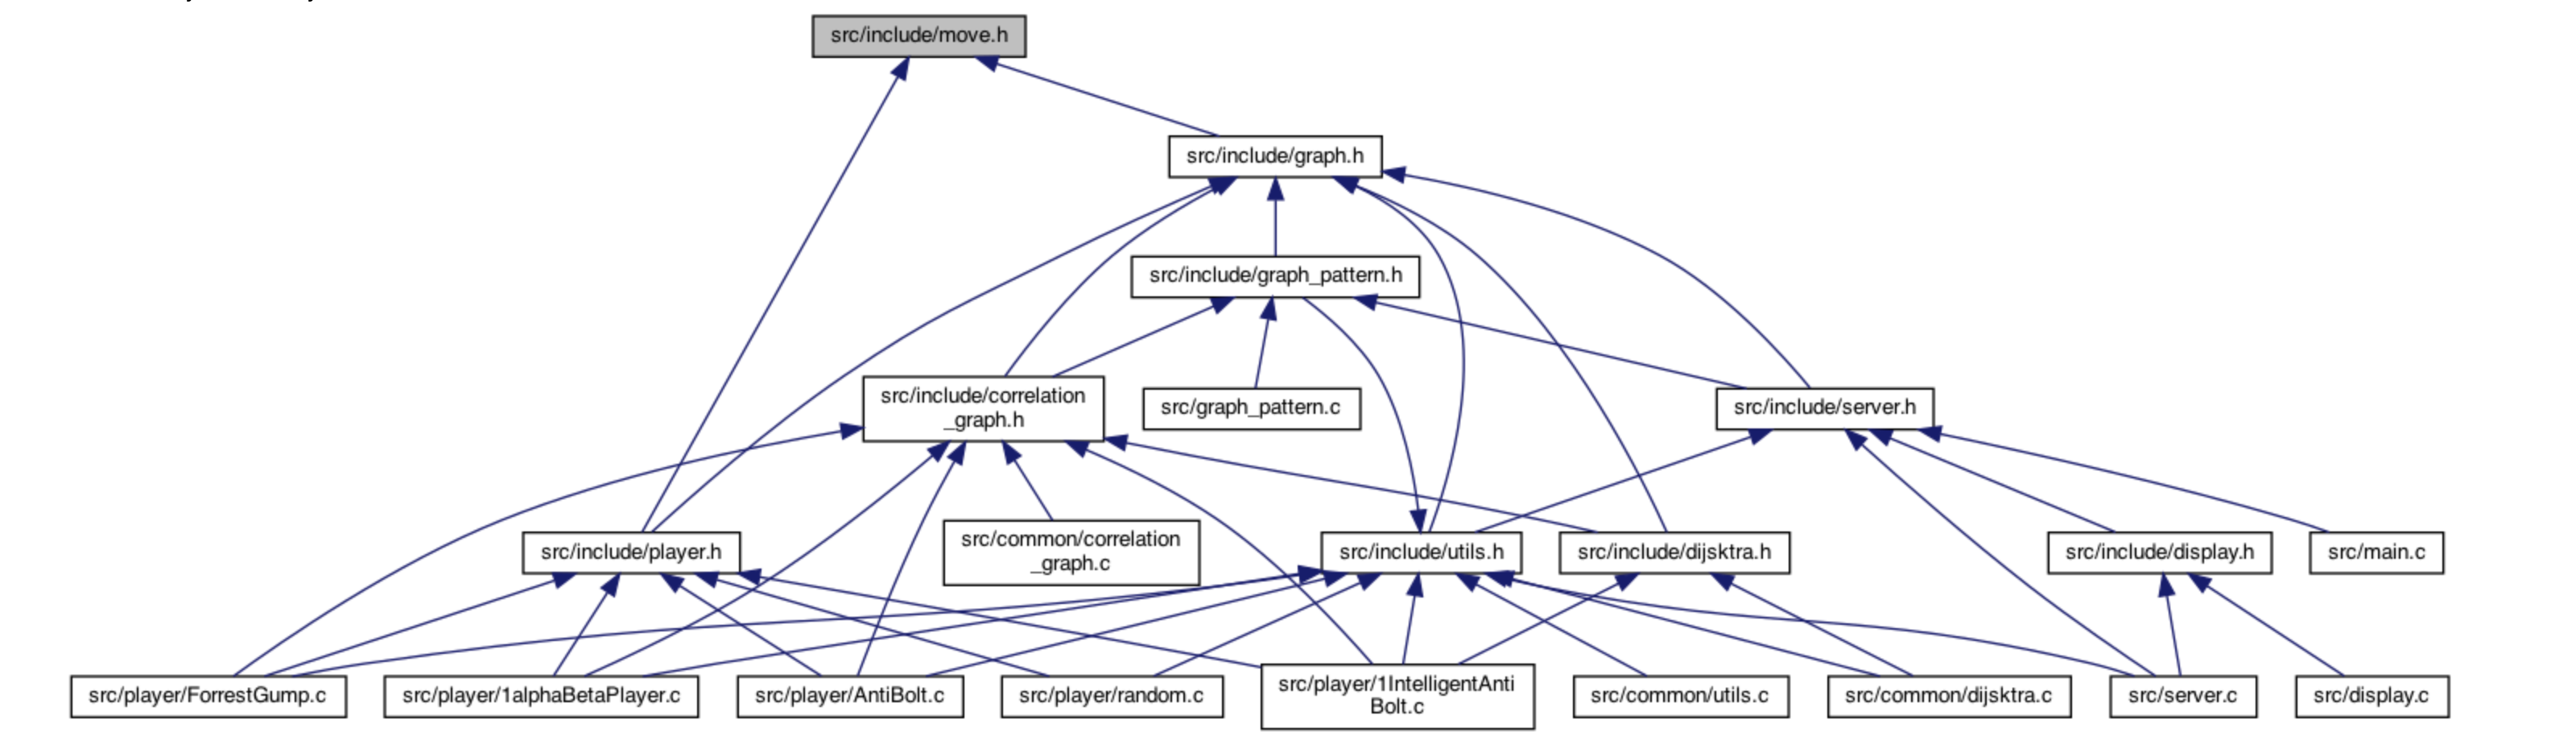
\includegraphics[width=\linewidth]{./dependency-graph.png}
    \caption{Graphe des dépendances du projet Quoridor}
    \label{fig:dependency-graph}
\end{figure}

\subsection{Améliorations possibles}
Notre projet est très interdépendant ce qui pourrait compliquer d'éventuelles ajouts ou modifications éventuelles. Pour améliorer cela, nous avons réfléchi à encapsuler la notion de serveur, d'affichage ou même de stratégie (afin d'avoir une fonction d'évaluation par stratégie et que le joueur puisse changer de stratégie si celle-là devient plus rentable) de manière à les rendre génériques et de ne plus s'attacher à leur implémentation, mais seulement à une interface commune. Par exemple, comme dit dans la partie \textit{amélioration possible} du serveur, nous n'avons pas besoin de connaître l'implémentation d'un serveur mais simplement d'avoir des fonctions servant d'interface telle que celle de l'initialisation, de la libération et de la mise en fonctionnement d'un serveur.\\

De plus, nous avons remarqué un manque de cohérence au niveau de l'ordonnancement des fichiers. En effet, si nous voulions respecter le critère de gestion des fichiers par thématique, alors le fichier source du serveur
aurait dû être dans un dossier et les fonctions permettant la création ou manipulation d'une \textit{structure  graph\_t} dans un autre dossier afin de ne laisser que le point d'entrée du programme, c'est-à-dire, le fichier main.c.\\

Une autre suggestion serait de mettre les fichiers en-têtes non plus dans le dossier \textit{include} mais à côtés de leur fichier source correspondant, car actuellement nous nous retrouvons avec des fichiers en-têtes de différents modules (\textit{player}, \textit{common}, ...) au même endroit. Les tests utilisent déjà cette pratique afin d'empêcher lors de la compilation de l'exécutable du jeu de possiblement prendre en compte des fonctions initialement non accessibles. En effet, afin de pouvoir réaliser différents tests unitaires, nous avons dû concevoir des fichiers en-têtes avec les différentes fonctions à tester à la base non accessibles.

\newpage
\section{Tests}

La politique des tests unitaires que nous avons effectuée est assez simple. Elle consiste à tester les cas extrêmes, puis certains cas plus généraux. Toutes les fonctions n'ont pas nécessité le même nombre de tests.

\subsection{Présentation de l'organisation du framework de tests}
Nous avons mis en place notre propre framework de tests avec des macros d'assertions basiques telles que : 
\begin{itemize}
    \item ASSERT\_TRUE, ASSERT\_FALSE : permet de vérifier une valeur de vérité;
    \item ASSERT\_EQUAL, ASSERT\_NOT\_EQUAL : permet de vérifier qu'une valeur est bien égale (resp. inégale) à une valeur attendue;
    \item ASERT\_NULL, ASSERT\_NOT\_NULL : permet de vérifier que le pointeur passé est \textit{NULL} ou non;
    \item ....
\end{itemize}

Nous avons ensuite mis en place un moyen de savoir si une assertion provoque une erreur ou si au contraire elle passe. Pour cela, nous obligeons les fonctions contenant des assertions d'avoir le prototype suivant : \texttt{int test\_nom\_du\_test();}.

Cela nous permet en cas d'erreur lors d'une assertion de retourner une valeur définie (ici $0$) et une autre si toutes les assertions sont passées (ici $1$). Une telle fonction  doit être lancée à partir de la macro \texttt{TEST\_FUNCTION} afin qu'elle soit bien prise en compte comme il le faudrait.

De plus, nous avons défini une macro \texttt{TEST\_FILE} permettant de lancer un regroupement de la macro \texttt{TEST\_FUNCTION} qui se trouve dans une fonction ayant pour prototype \texttt{void tests\_\_nom\_fichier\_functions();}. Cela permet de créer pour chaque fichier test une fonction lançant tous les tests de ce même fichier.

Un exemple de cette mise en place est visible à la figure \ref{fig:tests-framework}.

\begin{figure}[H]
    \centering
    \begin{minipage}{0.55\linewidth}
        \centering
        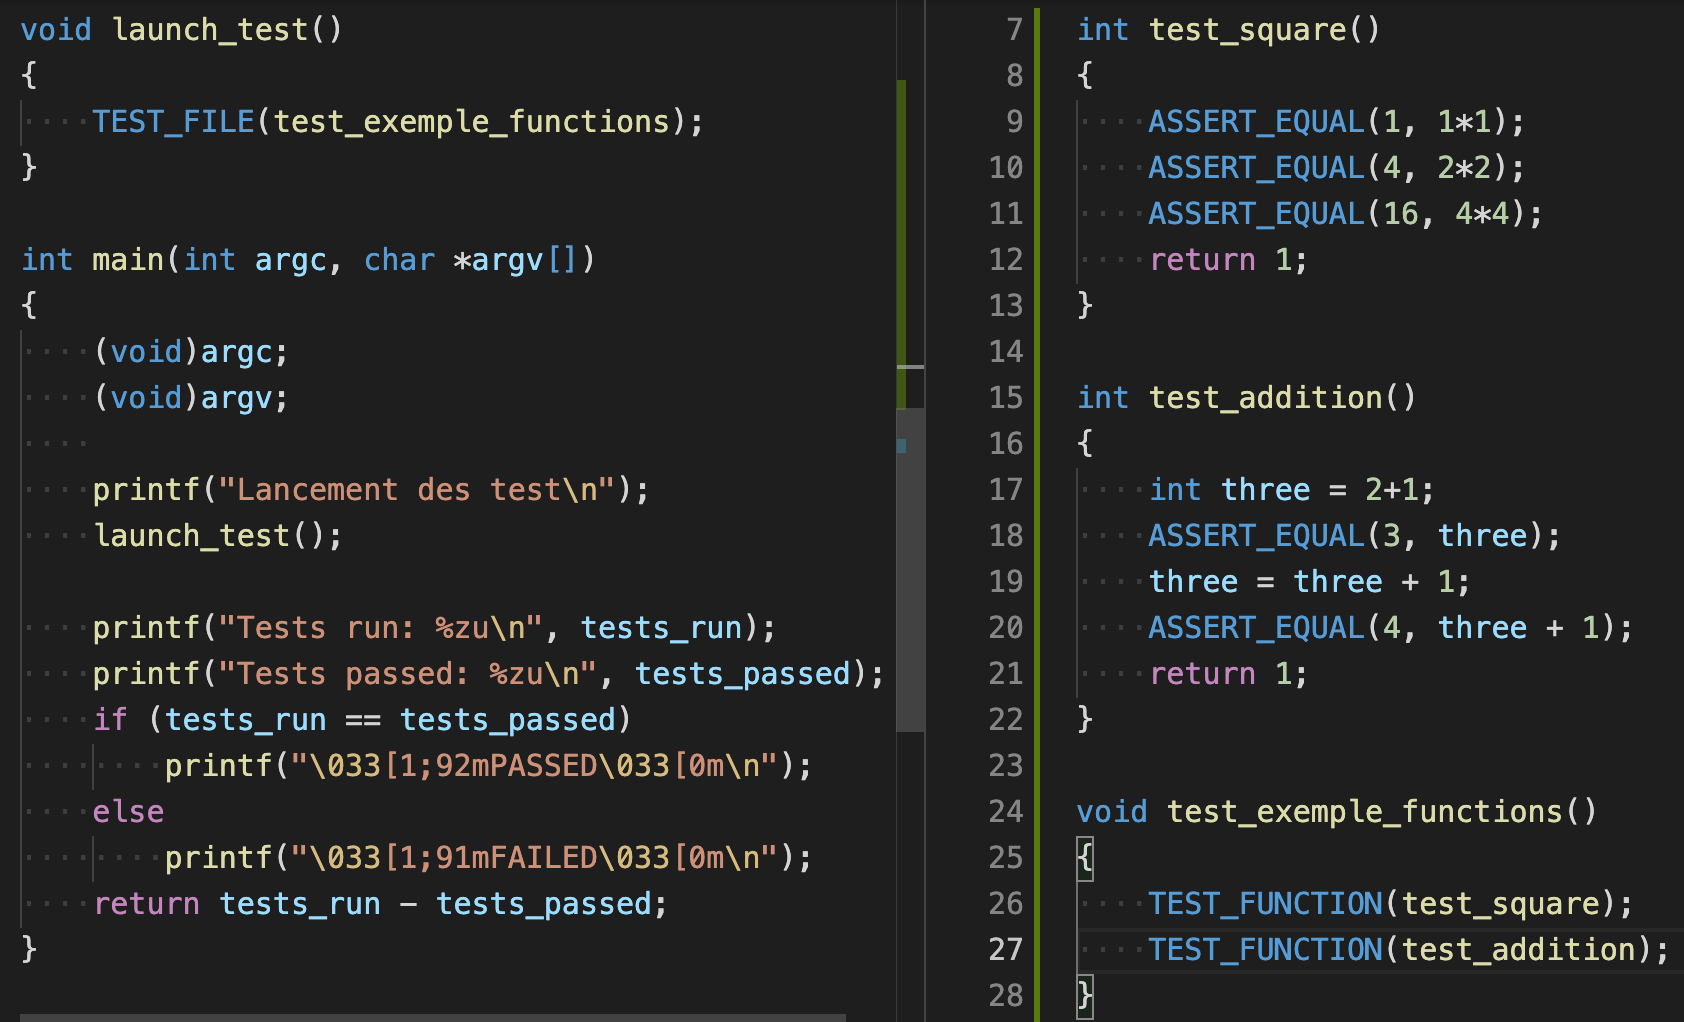
\includegraphics[width=1\linewidth]{test-framework-code.png}
    \end{minipage}
    \hfill
    \begin{minipage}{0.44\linewidth}
        \centering
        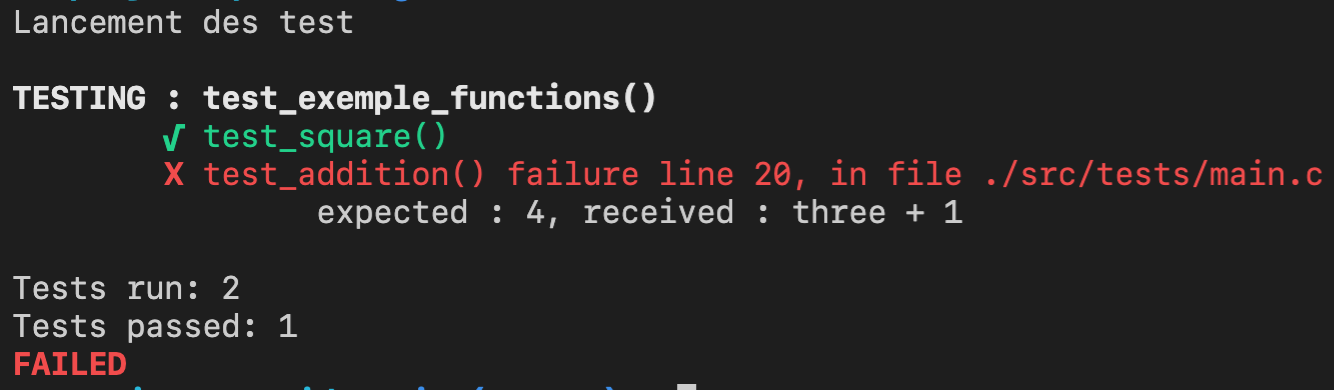
\includegraphics[width=1\linewidth]{test-framework-result.png}
    \end{minipage}
        \caption{Exemple simple de tests et de leurs résultats}
    \label{fig:tests-framework}
\end{figure}

\subsection{Tests des fonctions communes au serveur et aux joueurs}

Les tests des fichiers sources, \textit{utils.c, dijsktra.c, list\_dynamic.c, correlation\_graph.c} et \textit{queue.c}, implémentant les fonctions communes au serveur et aux joueurs ont été séparés en différents fichiers tests respectivement à leur nom, dans le sous-dossier \texttt{src/tests}. Ces tests unitaires vérifient le bon fonctionnement de chacune des fonctions y étant implémentées.

Par ailleurs, une partie du développement s'est aussi pilotée par les tests, notamment pour l'implémentation des fonctions de validation des coups des joueurs.

Ainsi, les tests réalisés ont permis d'obtenir des couvertures raisonnables, affirmant le bon fonctionnement des fonctions implémentées. Ces dernières sont résumées dans la table \ref{tab:coverage} suivant:

\begin{table}[H]
\begin{center}
\begin{tabular}{|c|c|}
\hline
Fichier source  & Couverture  \\ 

\hline

\textit{utils.c}         & $86.47$\% \\
\textit{dijkstra.c}      & $100$\% \\
\textit{list\_dynamic.c} & $100$\% \\ 
\textit{correlation\_graph.c} & $100$\% \\
\textit{queue.c} & $100$\% \\

\hline
\end{tabular}
\end{center}
\caption{\label{tab:coverage}Taux de couvertures des fichiers implémentant les fonctions communes au serveur et aux joueurs}
\end{table}

Les fonctions de \textit{utils.c} non testées sont les fonctions triviales \texttt{load\_library} et \texttt{load\_function} permettant la gestions des bibliothèques dynamiques, ainsi \texttt{get\_name\_type\_player}.

\subsection{Tests des joueurs}

Contrairement à l'utilisation classique de l'édition de lien pour la réalisation des tests, ceux des joueurs ont nécessité un chargement dynamique de leur fonctions, d'une manière similaire à celle utilisée lors du chargement dynamique par le serveur des différents clients. En effet, en raison de la contrainte de n'avoir qu'un seul exécutable \texttt{alltests} pour exécuter l'ensemble des tests des clients implémentés, il n'était alors pas possible d'appliquer une édition de lien classique aux tests des joueurs, ces derniers ayant au moins quatre fonctions de même noms, ce qui aurait impliqué des définitions multiples. Une autre solution viable mais qui n'a été proposé qu'à la fin aurait été de créer des bibliothèques dynamiques de test pour chaque joueur, de les charger puis de lancer les tests à l'intérieur de l'exécutable \texttt{alltests}.

\subsubsection{Test de la stratégie Random}

Le client random étant un client naïf très simple d'implémentation, nous avons simplement réalisé des tests sur la fonction de recherche des cases accessibles, puis sur la stratégie générale du joueur suivant plusieurs situations de départ. \\

Pour le premier test, nous mettons en place un graphe avec des murs, un adversaire, et nous appelons la fonction de recherche des positions disponibles. Nous pouvons alors comparer ce qu'elle retourne avec ce que nous attendons comme résultat. \\

En ce qui concerne la stratégie générale, nous positionnons le joueur dans des situations plus ou moins communes, puis nous testons l'action renvoyée par la fonction \texttt{play}. Nous regardons d'abord si l'action est légale, puis si elle correspond bien à un déplacement sur une case aléatoire parmi les cases disponibles. \\

Le taux de couverture n'étant pas calculable du fait du chargement dynamique de la bibliothèque, ces tests restent important pour vérifier la bonne réalisation de la stratégie. De plus, la visualisation des parties grâce à un affichage sur le terminal renforce l'idée du bon fonctionnement du client.

\subsubsection{Test de la stratégie Forrest Gump}

Le client Forrest Gump utilise des fonctions intermédiaires pour la mise en place de sa stratégie. Ainsi, les tests réalisés portent sur toutes ces fonctions secondaires qui servent à la création du déplacement envoyé au serveur. \\

Ainsi, après avoir testé la création d'un \texttt{struct move\_t} par la fonction \texttt{set\_move}, nous pouvons vérifier la fonction \texttt{get\_first\_move} qui renvoie une position aléatoire parmi les positions de départ. \\
Cependant, cette fonction n'est appelée que lorsque le joueur n'est pas encore positionné sur le plateau. Nous avons donc établi deux tests (positif et négatif) de la fonction \texttt{is\_first\_move}. \\

La stratégie Forrest Gump, comme expliqué en section \ref{sec:ForrestGump}, est une stratégie qui teste les 12 cases susceptibles d'être accessibles depuis une position dans un ordre de priorité. Nous avons donc réalisé des tests sur la fonction de classement de ces cases suivant la direction favorite du joueur. \\
Ainsi, il ne restait plus qu'à tester l'appel à la fonction \texttt{get\_new\_move} et de comparer le déplacement retourné par rapport à celui attendu en fonction de la stratégie qui vise à courir vers l'avant le plus vite possible.

\subsubsection{Test de \textit{IntelligentAntiBolt}}

Afin de tester ce joueur, nous avons réalisé plusieurs tests unitaires, mais aussi un test applicatif de déroulement de partie dans lequel plusieurs cas de configuration ont été testés. Tout d'abord nous avons vérifié que le nom du joueur renvoyé par la fonction \texttt{get\_player\_name} était le bon. Ensuite, les placements du joueur en début de partie ont été vérifiés pour différents types de graphes de tailles variables. Par la suite, nous avons testé les sorties de la fonction \texttt{can\_fast\_forward} pour différentes configurations. Puis finalement nous avons testé le comportement du joueur sur une partie où nous contrôlions le joueur adverse. Nous avons d'abord vérifié si \texttt{IntelligentAntiBolt} posait correctement les murs afin d'empêcher le joueur adverse d'aller tout droit pour gagner puis nous avons placé des murs pour tester si \texttt{IntelligentAntiBolt} empruntait le chemin le plus court pour gagner. Des tests impliquant les possibilités de sauter pour le joueur ont également été mis en oeuvre.

\subsubsection{Test de la stratégie Minimax}

Le comportement du joueur utilisant la stratégie Minimax étant plus complexe que celui des autres clients, son implémentation s'est servie de plusieurs fonctions intermédiaires, permettant conjointement la décision du coup à réaliser. 

\begin{figure}[H]
    \centering
    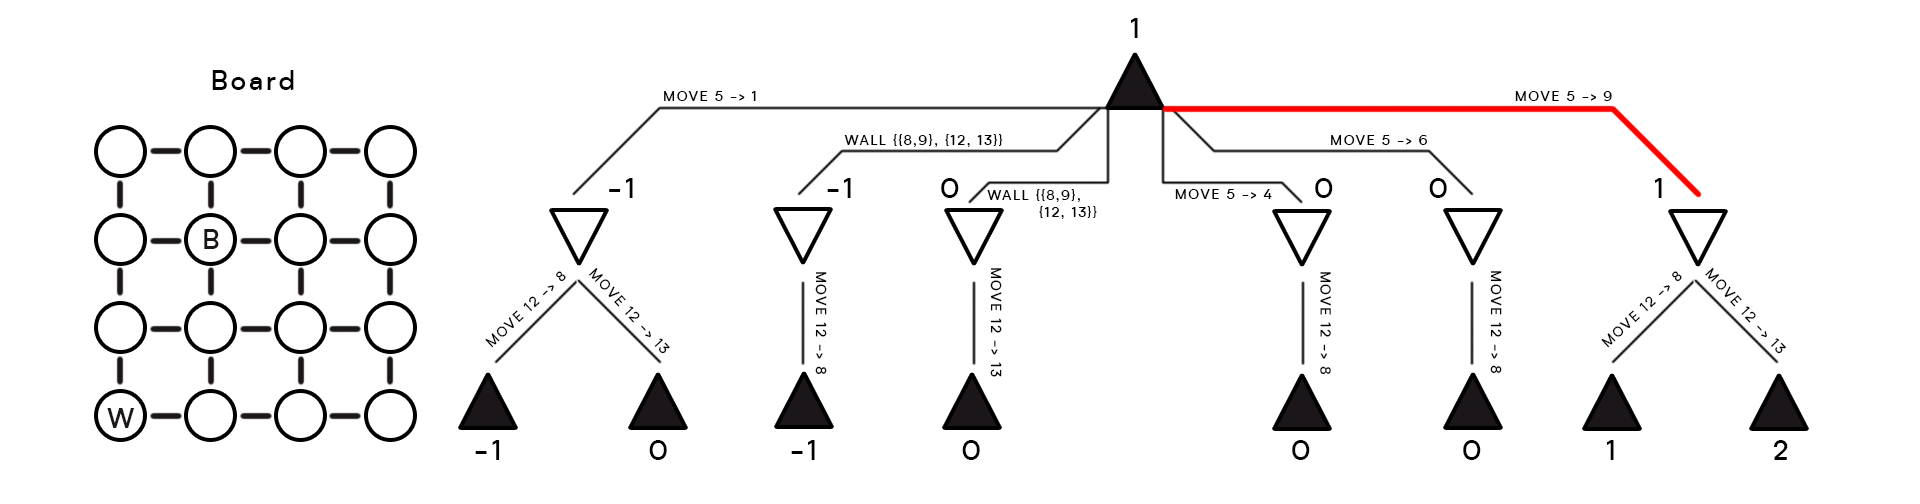
\includegraphics[width=\textwidth]{Tree_test.png}
    \caption{État de la partie utilisée lors d'un test de la stratégie Minimax et son arborescence issue de l'élagage Alpha-Beta}
    \label{fig:tree_test}
\end{figure}

Ainsi, à raison de ne pas pouvoir raisonnablement réaliser à la main des arborescences de jeu trop profonde, les recherches Minimax effectuées sont de profondeur $2$, permettant de couvrir les cas des joueurs maximisant et minimisant, tout en étant reproductibles sur papier. Le comportement de l'algorithme de Minimax a alors été vérifié dans des situations extrêmes de victoire ou de défaite évidentes, puis dans un cas général aboutissant à la comparaison des distances, et donc des scores d'utilités des feuilles obtenues à partir de l'arborescence de jeu, tel qu'illustré par la Figure \ref{fig:tree_test}. Les triangles noirs représentent le joueur noir maximisant (B), et les triangles blancs inversés le joueur blanc (W) minimisant. Dans cette situation, la valeur d'utilité remontant l'arbre est alors $1$, impliquant le choix de la branche rouge, i.e., un coup de type \texttt{MOVE} du sommet $5$ à $9$. Ce choix est alors cohérent avec l'état du plateau et les positions des joueurs sur le plateau.

Par ailleurs, le comportement des fonctions résolvant le problème du plus court chemin vers la zone adverse (\texttt{get\_distance\_between\_positions} et \texttt{get\_minimal\_distance\_to\_opponent\_area}), utilisant un algorithme de parcours en largeur, a été vérifié dans des situations avec ou sans murs, et sur un plateau torique. Ces mêmes fonctions régissent le comportement de la fonction d'évaluation \texttt{heuristic\_evaluation}, pour laquelle le comportement a aussi été vérifié dans des comportements extrêmes de victoire et défaite, mais aussi lors de situation impliquant la comparaison des distances de victoire pour chacun des joueurs. De plus, la vérification de l'élagage de l'ensemble des coups légaux possibles a aussi été contrôlée, permettant de tester le comportement final de \texttt{get\_legal\_moves} (de complexité celle de \texttt{can\_add\_wall}). Enfin, les fonctions triviales permettant d'obtenir le prochain état du jeu en conséquence d'un coup ont aussi été vérifiées, ces dernières étant essentielles au bon fonctionnement de l'algorithme de Minimax.

Bien que ne pouvant pas vérifier le taux de couverture (en raison du chargement dynamique des clients), l'ensemble de ces tests ont eu pour objectifs de tester la stratégie sous différents angles, permettant d'affirmer son bon comportement. De plus, les nombreuses parties réalisées en interne ou sur le Ladder permettent de soutenir cette même thèse.



\newpage
\section{Gestion de projet}
Dans cette section, nous présentons la manière dont nous avons managé le projet en terme de répartition des tâches ainsi que les améliorations possibles.

\subsection{Répartition des tâches}
Notre première approche consistait à se répartir le projet en deux groupes distincts. Le premier groupe se restreignait au développement du serveur tandis que le deuxième groupe à celui des joueurs. À ce moment-là, nous n'avions pas déterminé de responsable de projet ou de manager.

Cette approche a peu à peu évolué afin de reformer plusieurs groupes et d'attribuer des tâches et des fonctions à chaque personnes afin d'obtenir la répartition suivante :
\begin{itemize}
\item CHOURA Alexandre : programmeur des fonctions communes aux joueurs et au serveur ainsi que d'un joueur (stratégie MiniMax);
\item GUÉRIN Léo : programmeur intervenant au niveau du serveur (d'initialisation des graphes) et des joueurs (stratégies AntiBolt et IntelligentAntibolt);
\item MARAIS Lucas : programmeur attitré aux joueurs (random, ForrestGump, MiniMax et AntiBolt) ;
\item SORNAY Jean-François : coordinateur du projet, programmeur sur le serveur et les joueurs, réusineur du code.
\end{itemize}

Cette étape fut nécessaire, car nous manquions de communications et de mise en commun des différentes idées et implémentations. Cela nous a permis d'avancer avec une meilleure dynamique avec moins de conflits d'implémentation et de faire du réusinage de code plus rapidement. Toutefois, nous avons remarqué que ce changement est arrivé un peu tard.

\subsection{Améliorations possibles}

Comme dit précédemment, le changement d'organisation fut mis en oeuvre un peu tard ce qui nous a contraint à retravailler un grand pourcentage du code déjà écrit, ce qui aurait pu être évité.

De plus, peu de temps fut consacré à l'analyse des besoins du projet et surtout des stratégies. Cela nous a amené à beaucoup de duplication de code entre les différents joueurs.
Ce manque d'analyse des besoins se ressent au niveau de l'implantation de stratégie pour les joueurs tel que évoqué en section \textit{Améliorations possibles} des joueurs.

\newpage
\section{Conclusion}

La réalisation du projet Quoridor nous a permis de travailler en équipe, contrairement au projet du semestre 5, nous étions 4. La coordination était donc beaucoup plus importante, et nous l'avons rapidement mise en place. L'objectif du projet qui était la mise en place d'une architecture client-serveur a été mené à bien avec l'implémentation de cinq joueurs/clients différents, tous pouvant jouer les uns contre les autres grâce au serveur. \\

\'Egalement, la mise en place de stratégies efficaces a pris une place importante dans ce projet. Cela nous a permis d'exploiter plusieurs matières liées à la programmation avec notamment la programmation impérative avancée, l'algorithmique des graphes et l'environnement de travail. En effet, la manipulation des bibliothèques dynamiques, le débuggage, l'utilisation d'algorithmes complexes comme Dijskstra ou encore MinMax, et la manipulation du dépôt Git requière des compétences dans toutes ces matières. \\

Ce projet a donc été un excellent moteur pour se familiariser avec la notion de debug, la manipulation d'une architecture client-serveur et de mettre en pratique des connaissances provenant de matières plus théoriques tel que l'algorithmique de graphes.


\newpage

\nocite{*}
\bibliography{main} 
\bibliographystyle{ieeetr}

\section*{Annexe}

\begin{figure}[H]
    \dirtree{%
    .1 Projet Quorridor.
       .2 src/.
            .3 include/.
                .4 list.h \DTcomment{Derniers changements}.
                .4 graph.h.
                .4 move.h.
                .4 player.h.
                .4 display.h.
                .4 graph\_pattern.h.
                .4 server.h.
                .4 dijsktra.h.
                .4 utils.h.
                .4 correlation\_graph.h.
                .4 queue.h.
                .4 list\_dynamic.h.
            .3 common/.
                .4 dijsktra.c.
                .4 utils.c.
                .4 correlation\_graph.c.
                .4 queue.c.
                .4 list\_dynamic.c.
            .3 player/.
                .4 random.c.
                .4 ForrestGump.c.
                .4 AlphaBetaPlayer.c.
                .4 AntiBolt.c.
                .4 IntelligentAntiBolt.c.
            .3 tests/.
                .4 main.c.
                .4 test.h.
                .4 test\_files.h.
                .4 test\_queue.c.
                .4 test\_list.c.
                .4 test\_correlation\_graph.c.
                .4 test\_utils.c.
                .4 test\_dijsktra.[c-h].
                .4 test\_graph\_pattern.[c-h].
                .4 test\_server.[c-h].
                .4 test\_randomPlayer.c.
                .4 test\_ForrestGumpPlayer.c.
                .4 test\_alphaBetaPlayer.c.
                .4 test\_IntelligentAntiBolt.c.
            .3 display.c.
            .3 graph\_pattern.c.
            .3 server.c.
            .3 main.c.
       .2 install/.
       .2 doxyfile.
       .2 Makefile.
       .2 README.md.
    }
    \caption{Arborescence du dossier du projet Quorridor}
    \label{fig:files-tree-structure}
\end{figure}

\end{document}